\documentclass[a4paper,10pt,oneside,openany]{book}
\usepackage[utf8]{inputenc}
\usepackage{amsmath}
\usepackage{cancel}
\usepackage{amsfonts}
\usepackage{amssymb}
\usepackage{xcolor}
\usepackage{mathrsfs}
\usepackage{amsfonts}
\usepackage{amsmath}
\usepackage{mathtools}
\usepackage{centernot}
\usepackage{graphicx}
\usepackage{setspace}
\usepackage{geometry}
\usepackage{tcolorbox}
\usepackage{hyperref}
\usepackage{stackengine}
\usepackage{bm} %bold math
%%%%%%%%%%%%%%%%%%%%%%%%%%%%%%%%%%%%%%%%%%%%%%%%%%%%%%%%%%%%%%%%%%%%%%%%%%%%%%%%%%%%%%%%%%%%%%%%%%
\usepackage{multicol}

%%%%%%%%%%%%%%%%%%%%%%%%%%%%%%%%%%%%%%%%%%%%%%%%%%%%%%%%%%%%%%%%%%%%%%%%%%%%%%%%%%%%%%%%%%%%%%%%%%
\usepackage{listings}
\usepackage{color}
\usepackage{qtree}

\definecolor{dkgreen}{rgb}{0,0.6,0}
\definecolor{gray}{rgb}{0.5,0.5,0.5}
\definecolor{mauve}{rgb}{0.58,0,0.82}

\lstset{frame=tb,
  language=C++,
  aboveskip=3mm,
  belowskip=3mm,
  showstringspaces=false,
  columns=flexible,
  basicstyle={\small\ttfamily},
 %numbers=left,
  numbers=none,
  numberstyle=\tiny\color{gray},
  keywordstyle=\color{blue},
  commentstyle=\color{dkgreen},
  stringstyle=\color{mauve},
  breaklines=true,
  breakatwhitespace=true,
  tabsize=3,
  %xleftmargin=0.5cm
}
%%%%%%%%%%%%%%%%%%%%%%%%%%%%%%%%%%%%%%%%%%%%%%%%%%%%%%%%%%
\usepackage{graphicx}
\graphicspath{ {images/} }

\definecolor{grigio}{RGB}{179,179,179}
%\theoremstyle{plain}
\newtheorem{thm}{Teorema}[section]
\newtheorem{deff}{Definizione}[section]
\newtheorem{dimm}{Dimostrazione}[section]

\geometry{a4paper,top=1.5cm,bottom=1.5cm,left=2.5cm,right=2.5cm,%
heightrounded,bindingoffset=5mm}

\newcommand{\tb}[1]{\textbf{#1}}
\newcommand{\e}[1]{\textit{#1}}
\newcommand{\DEF}[1]{\textcolor{blue}{DEF:}}
\newcommand{\om}[0]{$\Omega$}
\newcommand{\al}[0]{$\mathcal{A}$}
\newcommand{\zero}[0]{$\emptyset$}
\newcommand{\ap}[0]{$\in$}
\newcommand{\im}[0]{$\implies$}

\setcounter{tocdepth}{1} %il grado di profondita indice, 1 solo chapter, 2 section ...

\author{Edoardo Lenzi}
\title{LFC (Linguaggi Formali e Compilatori) - Note del Corso}
\begin{document}
\maketitle
\tableofcontents
\chapter{Introduzione}
Un compilatore \'e un programma che legge un \textbf{linguaggio source} e lo traduce in un \texttt{equilvalente} \textbf{linguaggio di programmazione
target}. 
Solitamente il compilatore compila in \texttt{assembly} e poi un \textbf{assembler} produce codice macchina.
Se il target language \'e un programma eseguibile pu\'o processare input e produrre output.

Un \textbf{interprete} \'e un altro tipo di language processor, invece di tradurre il linguaggio lo esegue direttamente
quindi piglia sia il source program che gli input e processa l'output

Infine il \textbf{preprocessore} risolve le macro nel sorgente codificandole in linguaggio nativo (espandendole) prima di compilare.

\begin{quote}
Solitamente il compilato va pi\'u veloce mentre l`interprete ti da diagnosi piu accurate dato che esegue il codice.
Nel caso di Java compilo il sorgente in linguaggio intermedio \texttt{bytecode} che poi interpreto sulla JVM.
\end{quote}

Il \textbf{linker} \lq\lq linka\rq\rq\ assieme moduli e librerie dove ho riferimenti ad altri file (risolve gli indirizzi).
Il \textbf{loader} invece fa il merge in memoria per l'esecuzione.

%img4

\section{Front-End of the Compiler}
La \textbf{parte analitica} del processo di compilazione spacca la sorgente in parti costituenti e impone su di esse una struttura 
grammaticale (stile dtd); sfrutta questa struttura per creare una rappresentazione intermedia.
Se non passa la validazione grammaticale mi tira errori. Il sorgente viene storicizzato in
una struttura dati chiamata \textbf{symbol table}. 

\section{Back-End of the Compiler}
La \textbf{parte di sintesi} invece traduce il sorgente guardando la rappresentazione intermedia e la symbol table;
le parti di analisi e sintesi sono chiamate anche \textbf{front-end of the copiler} mentre le restanti \textbf{back-end}.

\section{Lexical analysis}
Fa uno scan e raggruppa le parole in \textbf{lexems}, per ogni lexem genera un \textbf{token} della forma

\begin{center}
    \texttt{(token name, attribute value)} 
\end{center}

Il \texttt{token name} \'e un simbolo astratto usato nella syntax analysis
mentre il \texttt{value} \'e un puntatore alla symbol table entry.\\[5pt]

\textbf{ie)}
\begin{quote}
    \texttt{position = initial + rate * 60} diventa \texttt{(id, 1) (=) (id, 2) (+) (id, 3) (*) (60)}\\
    gli operatori matematici sono simboli astratti che non hanno attribute value (?non sono referenziati nella symbol table?).
\end{quote}

%img7

\section{Session syntax analyzer} 
\'E un parsing, con i token crea una \textbf{rappresentazione ad albero (syntax tree)} nel quale 
il nodo \'e un operatore e i figli gli operandi. 

gli operatori devono avere priorit\'a per costruire l'albero, la struttura grammaticale serve anche a 
definire le priorit\'a degli operatori.

\section{Semantic analyzer} 
Piglia il \texttt{syntax tree} e guarda se \'e semanticamente consistente con la definizione del linguaggio.
(ie \texttt{type checking}). Il linguaggio puo ammettere cast impliciti chiamati \textbf{coercizioni} o tirare cogne.

\lq\lq \textit{intofloat}\rq\rq \'e una coercizione dell'intero 60 in float dato che gli altri operandi sono float. 

\section{Intermediate code generation}
Nel processo di compilazione posso avere varie rappresentazioni intermedie come alberi etc..
Dopo semantic analysis solitmente creo un codice basso livello, machine-like, \textit{\lq\lq easy to 
produce and esay to translate int target machine code\rq\rq}. Nella figura ho un tree address code
ricavato dal syntax tree. 

In un tree address code a destra ho al massimo un operatore (assembly like), e le operazioni sono in ordine.

Devo avere variabiline intermedie
\section{Code generation}
Segue la fase opzionale di \textbf{code optimization}, prende la rappresentazione intermedia e la mappa in un target language.
Le istruzioni intermedie vengono tradote in istruzioni macchina (presumibilmente). Devo capire come mappare variabili su registri

Nella symbol table devo storicizzare tutti gli attributi di un variable name.
 
Solitamente posso agglomerare le fasi di analisi in front end pass e le altre in back end pass.







\chapter{2}
Syntax descrive la forma appropriata di un programma 
Semantic descrive il significato...

Per specificare la sintassi uso BNF (Backus Naur Form) context-free grammar 

%img41

\textbf{Analisi} consiste nel (guardando la \textbf{sintassi}) spaccare il sorgente in parti costituenti (lexems) e generare tokens che li 
rappresentano (ho un linguaggio intermedio). La \textbf{Sintesi} invece parte dal linguaggio intermedio e sintetizza il target program.

Per specificare la \textbf{sintassi} uso la notazione della \textbf{context-free grammar} o BNF (Backus Naur Form).

%img
 
\section{Syntax Analysis}
Vedo una sequenza di caratteri come entit\'a chiamate tokens

%img

Creo un \textbf{abstract syntax tree} con entit\'a sulle foglie e operatori sugli altri nodi (intermedi).

\Tree [.assign a [.+ b c ] ]
\textbf{three address instruction} per via del fatto che ho tre variabili (istruzione assembly).

\begin{lstlisting}
    if(expression) statement else statement
    
    stmt -> if(expr) stmt else stmt
    // -> la traduco in "can have the form"
\end{lstlisting}

La regola sopra pu\'o essere chiamata \textbf{produzione}.

In una \textbf{produzione} elementi lessicali come if e parentesi (keywords) cono chiamati \textbf{terminali} mentre le variabili 
sono \textbf{non terminali} (ulteriormente espandibili con produzioni).

Una \textbf{context-free grammar} ha:
\begin{itemize}
    \item un \textbf{set di terminali} (tokens), set di simboli elementari del linguaggoi definiti dalla grammatica\\
    \item un \textbf{set di non terminali} o syntactic variables\\
    \item un \textbf{set di produzioni} ($Head \rightarrow Boby$)\\
        head \'e il costrutto, body la forma scritta del costrutto\\
    \item un non terminale chiamato \textbf{start symbol}\\
\end{itemize}

In un compilatore il lexical analyzer legge i caratteri del sorgente, li raggruppa in lexems e produce tokens 
(della forma \textbf{(TokenName, AttributeValue)}).

Specifico, nella pratica, una grammatica come lista di produzioni (con quelle contenenti lo start symbol per prime). 
Simboli come $<,\ >,\ =$ e le keyword del linguaggio sono terminali.

Per convenzione scrivo in \textit{italic i non terminali} ed in \textbf{boldface per i terminali}.
Uso l'operatore OR $|$ (pipeline) per separare gli elementi nel body. Definisco $\varepsilon$ come empty string.

\subsection{ie)}
ho $5+9-3+5-6-7+1$
\begin{lstlisting}
    list -> list + digit | list - digit | digit
    digit -> 0|1|2|...|9
\end{lstlisting} 
I terminali sono $\{+-0123...9\}$, i non terminali $\{list,\ digit\}$, start symbol \'e $list$

\section{Derivations}
Una grammatica deriva stringhe partendo dallo start symbol e ricorsivamente applicando le produzioni sui non terminali.
Il linguaggio definito da una grammatica \'e il $\{$stringhe ottenute$\}$.

\subsection{ie)}
\begin{lstlisting}
    //argomenti di una funzione
    call -> id(optparams)
    optparams -> params | Epsilon
    params -> params, param | param
\end{lstlisting}

\section{Parsing}
Il \textbf{parsing} \'e il problema secondo cui, data una stringa di terminali, devo capire come \'e stata costruita partendo da uno start 
symbol (tirare eccezione altrimenti).

Uso \textbf{parse trees} $A \rightarrow XYZ \implies$ \Tree [.A Y X Z ].

Regole di costruzione:
\begin{itemize}
    \item la root \'e lo start symbol\\
    \item le foglie sono terminali o $\varepsilon$\\
    \item i nodi interni sono non-terminali\\
    \item se A non-terminali ha figli $x_1,...,x_n \implies A \rightarrow x_1...x_n$ \\
\end{itemize}

9-5+2 \Tree [.list [.list [.l [.d 9 ] ] - [.d 5 ] ] + [.digit 2 ] ]

Una stringa pu\'o avere pi\'u parse tree ma ci\'o implica che la \textbf{grammatica \'e ambigua}; la presenza di pi\'u alberi implica 
l'esistenza di pi\'u significati diversi.

Mergiando le nozioni di list e digit ottengo 
$ string \rightarrow string + string | string - string | 1 | 2 | ... | 9$
9-5+1 ha 
\Tree [.string [.string [.string 9 ] - [.string 5 ] ] + [.string 2 ] ]
\Tree [.string [.string 9 ] - [.string [.string 5 ] + [.string 2 ] ] ]

\subsection{Associativit\'a a sinistra}
L'operatore + assicia a sinistra perch\'e se ho un pezzo di espressione $+ 5 +$ il + a sinistra viene applicato al 5 mentre ad esempio per 
l'elevamento a potenza o l'assengnazione di una variabile (=) l'associativit\'a \'e a destra (right associative).

\begin{lstlisting}
    a = b = c -> a = (b = c)
    2^3^4 -> (2^3)^4
    1 + 2 + 3 -> (1 + 2) + 3
\end{lstlisting}

Stringhe right associative (l'abero crese a destra) sono generate dalla grammatica:
\begin{lstlisting}
    right -> letter = right | letter
    letter -> [ab...z]
\end{lstlisting}

%img 72

\section{Precedenze degli operatori}
L'associativit\'a vale per operandi uguali ma non risolve $a + b * c$.
In questo caso ho due livelli di precedenza uno per $+-$ ed uno per $*/$.
Creo \textit{expr e term} per i due livelli e \textit{factor} per i base units.

\begin{lstlisting}
    factor -> digit | (expr)
    term -> term * factor
            | term / factor
            | factor
    expr -> expr + term
            | expr - term
            | term 
\end{lstlisting}
La grammatica sar\'a quindi 
\begin{lstlisting}
    expr -> expr + term | expr - term | term 
    term -> term * factor | term / factor | factor
    factor -> digit | (expr)
    // non posso avere un operatore vicino ad un fattore
\end{lstlisting}

\begin{tcolorbox}\begin{center}
    Posso generalizzare il concetto per n livelli di precedenza (per n livelli mi servono n+1 non terminali)
\end{center}\end{tcolorbox}

expr = list $\{$terms separati da $*/ \}$

\section{Java statements}
\begin{lstlisting}
    stmt -> id = expr
            | if (expr) stmt
            | if (expr) stmt else stmt
            | while (expr) stmt
            | do stmt while (expr)
            | {stmts}
    stmts -> stmts stmt
            | Epsilon
\end{lstlisting}

\subsection{ie) notazione postfissa}
\begin{lstlisting}
    //prefissa con     SS -> +SS|*SS|a
    SS -> SS+|SS*|a
    genera aa+a*
    S->SS*-> Sa*->SS+a*->aa+a*
\end{lstlisting}

\Tree [.S [.S [.S a ] [.S a ] + ] [.S a ] * ]

\subsection{ie) }
\begin{lstlisting}
    S -> 0S1 | 01
    000000111111
    0^n 1^n

    S -> S(S)S | E
    S -> S(S)S -> S(S)S(S)S -> S(S(S(S(S)S)S)S)S(S)S(S)S(S)S
    E(E(E(E(E)E)E)E)E(E)E(E)E(E)E
    avro' sempre una E(E all'inizio ed una E)E alla fine

    S -> aSbS | bSaS | E
    avro' sempre un numero uguale di a e b, lunghezza totale pari
\end{lstlisting}

%Esercizi pagina 74

\section{Syntax Directed Translation}
Fatte attaccando regole o frammenti di programma a produzioni.

\textbf{Attributi} sono propriet\'a di espressioni del linguaggio (length).

\textbf{Syntax Directed Translation Schemes} 

\subsection{Postfix notation} 
(ab+), 9-5+2 diventa 95-2+, 9-(5+2) diventa 952+-. La notazione postfissa non necessita di parentesizzazioni, non pu\'o avere ambiguit\'a.
Per leggere l'espressione faccio uno scan da destra fino al primo operatore e lo applico (vado avanti ricorsivamente).

\textbf{Syntax Directed Definition} associa 
\begin{itemize}
    \item ad ogni simbolo un set di \textbf{attributes}\\
    \item ad ogni produzione un set di \textbf{semantic rules} per computare i valori degli attributi associati ai simboli che 
        compaiono nella produzione\\
\end{itemize}

Per una stringa x faccio un \textbf{parse tree} poi applico le regole semantiche per valutare gli attibutes ad ogni nodo dell'albero.
x.a \'e l'attributo a di x $\rightarrow$ \textbf{annoted parse tree}

%img 77

Un attributo \'e detto \textbf{sintetizzato} se il suo valore in un nodo \'e determinato dai valori dei suoi figli e dal nodo stesso.
Un attributo \'e detto \textbf{inherited} se il suo valore in un nodo \'e determinato dai valori del padre, dei fratelli e di se stesso.

%img78

Uso l'operatore $||$ per concatenare le stringhe. Le regole semantiche sono applicate agli attributi.

\begin{lstlisting}
    expr -> term    =>  expr.t = term.t 
    expr -> expr1 + term    => expr.t = expr1.t || term.t || '+'
    // l'attributo nella head = attributi nel body concatenati con strighe extra ('+')
\end{lstlisting}

\section{Tree traversals}

\chapter{Progetto}
%https://sites.google.com/a/unitn.it/software-engineering-ii---designing-applications-that-matter/home
%https://github.com/marcorobol/is2-2017
%https://www.facebook.com/trentose2
%https://sites.google.com/site/sphoebss/project-definition
%https://sites.google.com/site/disibpm/

DOM struttura della pagina HTML 
JS mono-thread ma si comporta come multithread
devo installare nodeJs (verifico la presenza con \texttt{node -v}

Devo buttare tutto su heroku


%%%%%%%%%%%%%%%%%%%%%%%%%%%%%%%%%%%%%%%%%%%%%%%%%%%%%%%%%%%%%%%
\chapter{Application Design}
\section{The Design Process}
\subsection{Empathize Mode}
L'empatia \'e lo sforzo nel capire l'utente, le sue abitudini ed i suoi problemi per disegnare un app utile.

\subsection{Define Mode}
Creo un design in base a cosa ho appreso dal contesto umano.

\subsection{Ideate Mode}
La parte del processo in cui mi concentro nella creazione delle nuove idee. 
Vado nel profondo, cerco di definire tutto quello che mi serve per realizzare un mockup.

\subsection{Prototype Mode}
Per vedere qualcosa e risolvere problemi fondamentali di design. \lq\lq Fail early and cheaply!\rq\rq .

\subsection{Test Mode}
Una seconda occasione di confronto con l'utente.

\section{EDD Empathy Driven Design}
Empathy: the feeling that you understand and share another person's experience and emotions. 
The ability to share someone else's feeling.

%%%%%%%%%%%%%%%%%%%%%%%%%%%%%%%%%%%%%%%%%%%%%%%%%%%%%%%%%%%%%%%
\chapter{Agile Development}

\begin{tcolorbox}
	\begin{center}
		Kanban e Scrum
	\end{center}
\end{tcolorbox}

\begin{itemize}
	\item development process\\
	\item principali tipi di processo\\
	\item	processi agile (caratteristiche e pro)\\
	\item Scrum e Kanban (similitudini e differenze)\\
	\item	come definire, caratterizzare ed eseguire:\\
		\item[-] user stories\\
		\item[-] backlogs\\
		\item[-] sprints\\
	\item linkare backlogs a github issues\\
%%%%%%%%%%%%%%%%%%%%%%%%%%%%%%%%%%%%%%%%%%%%%%%%%%%%%%%%%%%%%%%%%%%%%%%%%
https://www.atlassian.com/agile
\section{What is agile}
\'E un approccio iterativo al project management e sw development;
molti piccoli incrementi (consegno il lavoro un pezzo alla volta). 
Tutti i piani, requisiti e risultati vengono rivisti spesso cos\'i da rendere 
il team resistente a cambiamenti in corso d'opera.

Il team si prende il controllo di come fare il lavoro, si autoorganizza per 
portare a termine task granulari.

\'E un set di tecniche di sviluppo accomunate dal continuo processo di 
miglioramento. Il manifesto Agile non da regole precise ma solo valori e 
linee guida che pongono le persone al primo posto.

\section{Il manifesto Agile}
http://agilemanifesto.org/iso/it/manifesto.html
siamo arrivati a considerare importanti:
\begin{itemize}
	\item \textbf{Gli individui e le interazioni} più che i processi e gli strumenti\\
	\item \textbf{Il software funzionante} più che la documentazione esaustiva\\
	\item \textbf{La collaborazione col cliente} più che la negoziazione dei contratti\\
	\item \textbf{Rispondere al cambiamento} più che seguire un piano\\
\end{itemize}

\subsection{I principi}
Seguiamo questi principi:

La nostra massima priorità è soddisfare il cliente
rilasciando software di valore, fin da subito
e in maniera continua.

Accogliamo i cambiamenti nei requisiti,
anche a stadi avanzati dello sviluppo.
I processi agili sfruttano il cambiamento
a favore del vantaggio competitivo del cliente.

Consegnamo frequentemente software funzionante,
con cadenza variabile da un paio di settimane a un paio di mesi,
preferendo i periodi brevi.

Committenti e sviluppatori devono lavorare insieme
quotidianamente per tutta la durata del progetto.

Fondiamo i progetti su individui motivati.
Diamo loro l'ambiente e il supporto di cui hanno bisogno
e confidiamo nella loro capacità di portare il lavoro a termine.

Una conversazione faccia a faccia
è il modo più efficiente e più efficace per comunicare
con il team ed all'interno del team.

Il software funzionante è il principale metro di misura di progresso.

I processi agili promuovono uno sviluppo sostenibile.
Gli sponsor, gli sviluppatori e gli utenti dovrebbero essere in grado
di mantenere indefinitamente un ritmo costante.

La continua attenzione all'eccellenza tecnica
e alla buona progettazione esaltano l'agilità.

La semplicità - l'arte di massimizzare la quantità
di lavoro non svolto - è essenziale.

Le architetture, i requisiti e la progettazione
migliori emergono da team che si auto-organizzano.

A intervalli regolari il team riflette su come
diventare più efficace, dopodiché regola e adatta
il proprio comportamento di conseguenza. 

\section{Aglie Frameworks}
Dal 2001 quando nasce il manifesto sono nati vari frameworks come Scrum, 
Kanban ed Extreme Programming (XP). Accomunati da iterazioni frequenti,
continuo imparare/aggiornarsi. 

\section{Project Management}
Un approccio iterativo per managing sw development projects, focalizzato 
su release continue e feedback continui. Il project management pu\'o essere 
categorizzato attraverso due frameworks: kanban e scrum.

\subsection{Scrum [Mischia]}
Fixed length iterations chiamati sprint.

ha 2 backlogs: 
	product backlog (lavoro che dev'essere fatto), ordinato per priorit\'a 
	sprint backlog, prendo gli issue dal prod backlog finchè la capacit\'a dello 
	sprint \'e saturata.

Nel team ci sono ruoli predefiniti:
	Scrum Master del team 
	Product Owner
	Scrum Team 

\subsection{Le quattro cerimonie}
Sprint Planning, meeting per capire quello che manca per finire lo sprint corrente
Sprint Demo, spiega cosa hanno realizzato nello sprint 
Daily StandUp, meeting di 15 minuti per sincronizzare il team 
Retrospective una review di cosa \'e andato bene e cosa migliorare

\subsection{Scrum Board}
To do, in progress, code review, done

\section{Kanban}
Focalizzato a fare le cose nel minor tempo possibile, mi permette di reagire 
a cambiamenti anche prima di Scrum. Non usa backlogs ma si focalizza solo 
sulla ToDo column questo permette di focalizzarsi su release continue che 
vengono fatte in qualunque momento.

Appena finisco qualcosa lo metto in done, il carico di lavoro sul team 
deve restare sotto il limite del WIP limit (un limite predefinito calcolato 
sulla capacit\'a del team) non posso superare con il lavoro in progress il 
WIP.

\subsection{Kanban four components}
stories (list of work) issues o task da fare
columns of lanes usate nella kanban board per distinguere diversi workstreams, users, projects, etc
Work In Progress limit limite calcolato sulla capacit\'a del team
Continuous Releases, il team lavora sulle stories sotto il limite WIP e pu\'o fare una release in qualsiasi momento.

\section{Estimated, Report and Plan}
Qualsiasi agile framework venga usato, devo visualizzare l'andamento del lavoro 
nel mio team per pianificare i futuri sprint.

In Kanban gli estimate sono molto importanti infatti il WIP si calcola sulle 
precedenti esperienze e team size. In Scrum mi serve per capire quanto lavoro 
posso fare nel prossimo sprint. 

Solitamente ad ogni task viene assegnato un peso per capire numericamente 
quanto ci metto. 
Le estimation vengono in gioco solo all'inizio/fine sprint; gli 
\textbf{agile report} mi da dei parametri del progresso dello sprint corrente 
(burndown charts) [basato sul numero di story points terminati].

\section{Grooming product backlog}
All'inizio di ogni sprint prendo dal backlog gli story points con priorit\'a maggiore,
il backlog \'e fondamentale proprio per avere una visione del progetto in toto, va mantenuto 
aggiornato.
%%%%%%%%%%%%%%%%%%%%%%%%%%%%%%%%%%%%%%%%%%%%%%%%%%%%%%%%%%%%%%%%%%%%%%%%%%%

http://leankit.com/
https://www.pivotaltracker.com/
Book: "Scrum: The Art of Doing Twice the Work in Half the Time"

https://www.proprofs.com/quiz-school/preview.php?title=ODM2MzUxL9VY
Sono in ritardo:
	lavoro extra
	consegno meno
	ritardo consegna (allungo lo sprint)
	allargo il team

Quale non è parte di scrum
	sprint planning meeting
	product review meeting
	sprint retrospective meeting

Principali differenze scrum e kanban 
Fasi del processo Scrum

%%%%%%%%%%%%%%%%%%%%%%%%%%%%%%%%%%%%%%%%%%%%%%%%%%%%%%%%%%%%%%
\chapter{Versioning and Collaboration}
git commands:
	init - how to start an empty repo
	clone
	status
	log
	checkout
	diff
	add - and why we have a staging area, how to use it
	commit - and commit strategies, when it is proper to commit
	merge - and solving merge conflicts
	branch - and when to branch/merge
	pull, push
	remote - setting up a remote repository
	rebase - and why/when to use it
	reset (and reset hard): when and how to revert to a state
	stash
	how/why to fork and perform pull requests

[GIT CLI]
https://www.atlassian.com/git/tutorials/what-is-version-control#benefits-of-version-control

[PR]
https://help.github.com/articles/about-pull-requests/


%%%%%%%%%%%%%%%%%%%%%%%%%%%%%%%%%%%%%%%%%%%%%%%%%%%%%%%%%%%%%%
\chapter{Testing}

	Black box and white box testing 
	TDD
	Jest 
	debugging and the bug lifecycle
\subsection{Jest}

https://facebook.github.io/jest/

To activate coverage insert this into your package.json:
\begin{lstlisting}
	"jest": {
		"verbose": true,
		"collectCoverage": true
	},
\end{lstlisting}

how to test asynch code, and how to perform setup and teardown

\section{Domande Utili}
Scopo di Regression Testing?
	Pu\'o sostituire Acceptance testing
	Ci consente di riutilizzare i test per massimizzare quindi iil ROI
	Riduce il lavoro di code review necessario quando modifico il codice
	Utile per scoprire bug introdotti come risultato di modifiche al codice ()

Quali sono i pro ed i contro di lasciare tutte le asserzioni a "on" nel codice in produzione
	[easier debugging, and failures are often better than bad data. 
cons: possibly, performances and possibly that they are not "friendly" (they crash the program) ]

For the following piece of code, how many test cases are needed to get 100% statement coverage:
Read (Colour) // Input colour from user
IF (Colour == “Red”) THEN
    Call Roses(Colour)
ELSEIF (Colour == “Blue”) THEN
    Call Violets(Colour)
ELSE
    PRINT “User is no Shakespeare”
SaveToDatabase(Colour)

(3 test)

Cosa si intende per unit testing?

\section{Esercizi}
For the below,

    Write the function,
    write test cases for it, based on black box testing and equivalence partitioning and boundary analysis
    write test cases to achieve 100% coverage

    Function that computes the square root of a positive number
    Function that receives four positive integers and returns if these integers can be the length of the sides of a rectangle. 
    Function that receives three positive integers and returns if these integers can be the length of the sides of a triangle, and also returns which kind of a triangle this is. 

Given this function, achieve

    E1: 100% statement coverage
    E2: 100% branch coverage


%%%%%%%%%%%%%%%%%%%%%%%%%%%%%%%%%%%%%%%%%%%%%%%%%%%%%%%%%%%%%%
\chapter{App design and Specs}

ApiAry/OpenApi
Cos'\'e una API, perch\'e hanno un ruolo centrale al giorno d'oggi,
come disegnare ed esporre una api.


%%%%%%%%%%%%%%%%%%%%%%%%%%%%%%%%%%%%%%%%%%%%%%%%%%%%%%%%%%%%%%
\chapter{Web Labs}

Consuming REST APIs from Node.js
	https://www.rapiddg.com/blog/calling-rest-api-nodejs-script
Authentication
	https://scotch.io/tutorials/authenticate-a-node-js-api-with-json-web-tokens
	https://stackoverflow.com/questions/319530/restful-authentication

%%%%%%%%%%%%%%%%%%%%%%%%%%%%%%%%%%%%%%%%%%%%%%%%%%%%%%%%%%%%%%
\chapter{Esame}
Domande di teoria
Pratica
Progetto
\section{Esercizio 1}
Create un servizio che riceve consegne di esami dagli studenti (e, in generale, a "workers" di consegnare "assignments". il servizio consente ad un worker di mandare il proprio assignment (esame), caratterizzato da:
	taskID - a string 
	assignmentID - a string
	workerID - a string
	assignmentResult - an object

gli utenti possono anche modificare un assignment consegnato, guardare assignments, e cancellare assignments (ovvero ritirarsi).
non implementiamo metodi di controllo degli accessi: per semplificare assumiamo che tutti possano fare tutto.

vi chiediamo di:

    definire API su apiary, almeno per la parte di gestione di assignments
    fare deploy su heroku del servizio, a cui l'host su apiary deve puntare
    mettere su github 
        il codice realizzato per implementare il servizio, in nodejs
        i casi di test, in jest, che testano tramite chiamate http(s)
    "consegnare" (chiamando una API che vi sara' fornita o inserendo gli url di apiary, github e heroku nella form indicata) dando gli URL relativi ad apiary, github repo, e heroku app

RIcordiamo di non modificare nulla dopo la consegna.

NON e' necessario memorizzare le info in un database.
Per i casi di test, basta mettere casi di test che testano un casi valido di get, di post, e di delete

Concentratevi sul fare poche funzionalita' fatte bene (ad es, un paio di metodi di API descritti bene, una o due funzioni implementate come si deve, una serie di casi di test per un metodo o due pensati bene con equivalence partitioning e boundary value analysis, magari anche con coverage se avete il tempo)

\subsection{Soluzioni}
https://examware.docs.apiary.io/
https://github.com/sphoebs/examware.git

\subsection{Varianti}
\begin{itemize}
	\item scrivere i casi di test raggiungendo 100$\%$ coverage (statement, branch,...)\\
	\item creare branch specifiche (ad es, una branch per una get, una branch per una put.... ) e di utilizzare una determinata branching strategy, o usando rebase\\
	\item creare stories su waffle per un problema complesso (di cui poi magari vi chiediamo implementazione di una piccola parte)\\
  \item potremmo partire da una codebase esistente e chiedere di capirla e modificarla. \\
  \item risolvere dei conflitti su merge\\
  \item creare remotes su git a varie sources, fare pull requests, creare issues su github analizzare le differenze con diff....\\



\chapter{Text Processing Tools}


\chapter{Analisi Sintattica}
$S \rightarrow cAd$
$A \rightarrow ab | a$

%%%%%%%%%%%%%%%%%%%%%%%%%%%%%%%%%%%%%%%%%%%%%%%%%%%%%%%%%%%%%%%%%%%%%%%%%%%%%%%%%%%%%%%%%%%%%%%%
\section{Parsing Top-down}
Parto dal starting symbol ed espando le derivazioni dando priorit\'a alle derivazioni pi\'u a sinistra.
Cerco quindi di ricostruire una derivazione leftmost della stringa w data in input.

$w\$, \$ \not\in V$\\
$w=cabd$

Per ricostruire la parola w parto dalla prima derivazioine $S \rightarrow cAd$ derivo la A pi\'u a sinistra (leftmost) e posso scegliere 
fra $a$ ed $ab$; scelgo $a$ e mi accorgo che ho sbagliato, torno in dietro e scelgo $ab$.

%%%%%%%%%%%%%%%%%%%%%%%%%%%%%%%%%%%%%%%%%%%%%%%%%%%%%%%%%%%%%%%%%%%%%%%%%%%%%%%%%%%%%%%%%%%%%%%%
\section{Parsing Top-down predittivo (o non ricorsivo)}
Cambio la grammatica sopra in: 
$S \rightarrow cAd$
$A \rightarrow aB$
$B \rightarrow b | \varepsilon $
Cos\'i non sbaglio 

%%%%%%%%%%%%%%%%%%%%%%%%%%%%%%%%%%%%%%%%%%%%%%%%%%%%%%%%%%%%%%%%%%%%%%%%%%%%%%%%%%%%%%%%%%%%%%%%
\subsection{Grammatica LL(1)}
prima L: leggiamo la input string da sinistra\\
seconda L: ricostruiamo una leftmost derivazione\\
(1): decidiamo quale operazione effettuare guardando un solo simbolo in input\\
Le grammatiche LL(1) sono un subset delle grammatiche libere.

\section{Algoritmi di Parsing}
\begin{tabular}{lc}
    input buffer    &   w$\$$   \\
    stack           &   bottom[$ \$ \qquad $] top \\
    parsing table   & con tante righe quante non terminali, tante colonne quante terminali ($ \$ $ incluso)\\
                    & in ogni cella metto un'eventuale trasformazione o \lq\lq error \rq\rq \\
\end{tabular}

%%%%%%%%%%%%%%%%%%%%%%%%%%%%%%%%%%%%%%%%%%%%%%%%%%%%%%%%%%%%%%%%%%%%%%%%%%%%%%%%%%%%%%%%%%%%%%%%
\subsection{Algoritmo di parsing non-ricorsivo}
\begin{center}
    \begin{tabular}{ll}
        input   &   stringa w, tabella parsing non ricorsivo T, per G\\
        output  &   derivazione leftmost di w se $w \in L(G)$, error() altrimenti\\
    \end{tabular}
\end{center}

\begin{lstlisting}
    //init
    buffer = {w$};
    stack.push($S);

    let b il primo simbolo di w 
    let x il top dello stack 

    while(x != $){
        if(x == b){
            pop(x);
            let b il simbolo necessario di w;
        } else if(x e'' terminale){
            error();
        } else if(T[x,b] contiene X -> Y1...Yn){
            return X -> Y1...Yn;
            pop(x);
            push(Yn...Y1)
        }
        let x il top dello stack
    }
\end{lstlisting}

%%%%%%%%%%%%%%%%%%%%%%%%%%%%%%%%%%%%%%%%%%%%%%%%%%%%%%%%%%%%%%%%%%%%%%%%%%%%%%%%%%%%%%%%%%%%%%%%%%%%%%%%%
\subsection{Esempio}
$E \rightarrow TE'$ \\
$E' \rightarrow +TE'|\varepsilon$\\
$T \rightarrow FT'$\\
$T' \rightarrow *FT'|\varepsilon$\\
$F \rightarrow id$\\

\begin{tabular}{|c|c|c|c|c|}
    \hline
            &   id                      &   +                           &   *   &   $\$$    \\
    \hline
        E   &   $E \rightarrow TE'$     &                               &     &      \\
    \hline
        E'  &                           &   $E' \rightarrow TE'$        &     &   $E' \rightarrow \varepsilon $    \\
    \hline
        T   &   $T \rightarrow FT'$     &                               &      &      \\
    \hline
        T'  &                           &   $T' \rightarrow \varepsilon$    &   $T' \rightarrow *FT'$   &   $T' \rightarrow \varepsilon$    \\
    \hline
        F   &   $F \rightarrow id$      &                               &      &       \\
    \hline
\end{tabular}

\begin{tabular}{|c|c|c|}
    \hline
    pila & input & output \\
    \hline
    $\$ $\underline{E}  &   \underline{id}+id*id$ \$ $  &   $E \rightarrow TE'$ \\
    \hline
    $\$ $ E \underline{T'}  &   &   $E \rightarrow TE' $ \\
    \hline
    $\$ ET'$\underline{F}  &   &   $F \rightarrow id $ \\
    \hline
    $\$ $ ET' \underline{id}  &    &   \\
    \hline
    $\$ E'$\underline{T''}  &  +\underline{id}*id $\$$  &   $T'' \rightarrow \varepsilon $ \\
    \hline
    $\$ $\underline{E'}  &    &   $E' \rightarrow TE'$ \\
    \hline
    $\$ $ E'T \underline{+}  &   \underline{id}*id$ \$ $  &   \\
    \hline
    $\$ $ E'\underline{T}  &     &   \\
    \hline
        &     ...Avanti cos\i     &   \\
    \hline
\end{tabular}

\Tree[.E [.T [.F id ] [.T' $\varepsilon$ ] ] [.E' + [.T  [.F id ] [.T' * [.F id ] [.T' $\varepsilon$ ] ] ] [.E' $\varepsilon$ ] ] ]

%%%%%%%%%%%%%%%%%%%%%%%%%%%%%%%%%%%%%%%%%%%%%%%%%%%%%%%%%%%%%%%%%%%%%%%%%%%%%%%%%%%%%%%%%%%%%%%%
\subsection{Esercizio}
$S \rightarrow aA | bB$\\
$A \rightarrow c $\\
$B \rightarrow d $\\

$w = ac\$ $ \\

Parsing: $S \implies aA \implies ac $\\

Nella tabella metto le produzioni della grammatica:

\begin{tabular}{|l|l|l|l|l|l|}
        &   a   &   b   &   c   &   d   &   $\$$    \\
    S   &   $S \rightarrow aA$   &    $S \rightarrow bB$   &      &      &      \\
    A   &      &      &  $A \rightarrow c$     &      &      \\
    B   &      &      &       &  $B \rightarrow d$    &      \\  
\end{tabular}

%%%%%%%%%%%%%%%%%%%%%%%%%%%%%%%%%%%%%%%%%%%%%%%%%%%%%%%%%%%%%%%%%%%%%%%%%%%%%%%%%%%%%%%%%%%%%%%%
\section{Calcolo First}
Data una generica $\alpha \in V^*$ per G=(V, T, S, P), first($\alpha$) \'e l'insieme dei simboli terminali b tali che $\alpha \implies bv$.
Inoltre se $\alpha \implies \varepsilon $ allora $\varepsilon \in first(\alpha )$

%%%%%%%%%%%%%%%%%%%%%%%%%%%%%%%%%%%%%%%%%%%%%%%%%%%%%%%%%%%%%%%%%%%%%%%%%%%%%%%%%%%%%%%%%%%%%%%%
\subsection{Esercizio}
$S \rightarrow A|B$\\
$A \rightarrow a|C$\\
$C \rightarrow \varepsilon$\\
Allora first(A) = $\{ a, \varepsilon \}$ ($\varepsilon$ perch\'e posso fare $A \implies C \implies \varepsilon $). 

%%%%%%%%%%%%%%%%%%%%%%%%%%%%%%%%%%%%%%%%%%%%%%%%%%%%%%%%%%%%%%%%%%%%%%%%%%%%%%%%%%%%%%%%%%%%%%%%
\subsection{Esercizio}
$S \rightarrow A|B$\\
$A \rightarrow a|C$\\
$C \rightarrow bB$\\
Allora first(A) = $\{ a, b \}$ (b perch\'e posso fare $A \implies C \implies bB$, ma B non esiste). 

%%%%%%%%%%%%%%%%%%%%%%%%%%%%%%%%%%%%%%%%%%%%%%%%%%%%%%%%%%%%%%%%%%%%%%%%%%%%%%%%%%%%%%%%%%%%%%%%
\subsection{Esercizio}
$S \rightarrow A|B$\\
$A \rightarrow a|C$\\
$C \rightarrow bB$\\
$B \rightarrow c$\\
Allora first(A) = $\{ a, b \}$ ($A \implies C \implies bB \implies bc$, ma tengo solo il primo simbolo (b)) 

%%%%%%%%%%%%%%%%%%%%%%%%%%%%%%%%%%%%%%%%%%%%%%%%%%%%%%%%%%%%%%%%%%%%%%%%%%%%%%%%%%%%%%%%%%%%%%%%
\subsection{Esercizio}
$A \rightarrow A|C$\\
$C \rightarrow bB|\varepsilon$\\
$B \rightarrow c$\\
Allora first(A) = $\{ a, b, \varepsilon\}$

G=(V,T,S,P)
Sia $X \in V$. L'insieme first(X) viene calcolato come segue:
\begin{itemize}
    \item[1)] inizializzo first(X) vuoto $\forall\ X \in V$\\
    \item[2)] se $X \in T$ allora first(X) = $\{ X \}$\\
    \item[3)] se $X \rightarrow \varepsilon \in P$ allora aggiungere $\varepsilon$ ai first(X)\\
    \item[4)] se $X \rightarrow Y_1...Y_n \in P$, con $n \geq 1$ allora uso la seguente procedura:\\
\end{itemize}
\begin{lstlisting}
    j = 1;
    while(j <= n){
        aggiungere ai first(X) ogni b tale che b in first(Yj)
        if(epsilon in first(Yj)){
            j++;
        } else {
            break;
        }
    }

    if(j == n+1){
        aggiungere epsilon ai first(X);
    }
\end{lstlisting}

Sia $\alpha=Y_1 ... Y_n,\ n\geq 1$, allora first($\alpha$) \'e calcolato sotituendo a X alpha:
\begin{lstlisting}
    j = 1;
    while(j <= n){
        aggiungere ai first(alpha) ogni b tale che b in first(Yj)
        if(epsilon in first(Yj)){
            j++;
        } else {
            break;
        }
    }

    if(j == n+1){
        aggiungere epsilon ai first(alpha);
    }
\end{lstlisting}

%%%%%%%%%%%%%%%%%%%%%%%%%%%%%%%%%%%%%%%%%%%%%%%%%%%%%%%%%%%%%%%%%%%%%%%%%%%%%%%%%%%%%%%%%%%%%%%%%%%%%%%
\subsection{Esercizio}
$E \rightarrow T E'$\\
$E' \rightarrow +T E' | \varepsilon $\\
$T \rightarrow FT'$\\
$T' \rightarrow *FT'| \varepsilon $\\
$F \rightarrow (E)|id $\\

First:
$E = \{ id, ( \}$ ovviamente ha gli stessi first di T per $E \rightarrow T E'$\\
$E' = \{ +, \varepsilon \}$\\
$T = \{ id, ( \}$ ha gli stessi first di F per $T \rightarrow FT'$\\
$T' = \{ *, \varepsilon \}$\\
$F = \{ id, ( \}$\\

Per generare id + id: \Tree[.E [.T [.F id ] [.T' $\varepsilon$ ] ] [.E' + [.T [.F id ] [.T' $\varepsilon$ ] ] [.E' $\varepsilon$ ] ] ]\\

Mancano le parentesi fra i terminali nella tabella...
\begin{tabular}{|c|c|c|c|c|}
    \hline  
        &   id                              &   +   &   *   &   $\$$    \\
    \hline  
    E   &   $E \rightarrow T E'$            &       &       &   \\
    \hline  
    E   &   &   $E' \rightarrow T E'$       &       &   $E' \rightarrow \varepsilon $ \\
    \hline       
    T   &   $T \rightarrow FT'$             &       &       &   \\     
    \hline   
    T'  &   &  $T' \rightarrow \varepsilon $   &   $T' \rightarrow *FT'$    & $T' \rightarrow \varepsilon $  \\   
    \hline    
    F   &   $F \rightarrow id $             &       &       &   \\    
    \hline  
\end{tabular}

%%%%%%%%%%%%%%%%%%%%%%%%%%%%%%%%%%%%%%%%%%%%%%%%%%%%%%%%%%%%%%%%%%%%%%%%%%%%%%%%%%%%%%%
\section{Follow}
$\forall\ A \in V \backslash T, $ follow(A):
\begin{lstlisting}
    follow(A) = emptySet per ogni A in (V \ T);
    follow(S).push($);

    repeat{
        foreach(B -> alpha A beta in P){
            if(beta == epsilon){
                follow(A).push(follow(B));
            } else {
                follow(A).push(first(beta) \ epsilon);
                if(epsilon in first(beta)){
                    follow(A).push(follow(B));
                }
            }
        }
    } until (saturazione);
\end{lstlisting}

%%%%%%%%%%%%%%%%%%%%%%%%%%%%%%%%%%%%%%%%%%%%%%%%%%%%%%%%%%%%%%%%%%%%%%%%%%%%%%%%%%%%%%%
\subsection{Esempio}

$S \rightarrow aABb$\\
$A \rightarrow Ac|d$\\
$B \rightarrow CD$\\
$C \rightarrow e|\varepsilon$\\
$D \rightarrow f|\varepsilon$\\

\begin{tabular}{ccc}
              &   First                     &   Follow      \\    
    $S=$      &    $\{ a \}$                &   $\{ \$ \}$        \\
    $A=$      &    $\{ d \}$                &   $\{e,f,b$ (da $S \rightarrow aABb$), c (da $A \rightarrow Ac$)$\}$ \\
    $B=$      &    $\{ e,f,\varepsilon \}$     &   $\{b \text{ (da } S \rightarrow aABb)\}$   \\
    $C=$      &    $\{ a,\varepsilon \}$       &   $\{f \text{ (da } B \rightarrow CD)\}$      \\
    $D=$      &    $\{ f,\varepsilon \}$       &   $\{\}$      \\
\end{tabular}

%%%%%%%%%%%%%%%%%%%%%%%%%%%%%%%%%%%%%%%%%%%%%%%%%%%%%%%%%%%%%%%%%%%%%%%%%%%%%%%%%%%%%%%
\subsection{Esempio}

$S \rightarrow aA|aBc$\\
$A \rightarrow Bd|Cc$\\
$B \rightarrow e|\varepsilon$\\
$C \rightarrow f|\varepsilon$\\

\begin{tabular}{ccc}
              &   First                   &   Follow            \\    
    $S=$      &    $\{ a, b \}$           &   $\{ \$ \}$        \\
    $A=$      &    $\{ e,d,f,c \}$        &   $\{ \$,(?) \}$    \\
    $B=$      &    $\{ e,\varepsilon \}$     &   $\{ c,d \}$       \\
    $C=$      &    $\{ f,\varepsilon \}$     &   $\{ c \} $        \\
\end{tabular}

%%%%%%%%%%%%%%%%%%%%%%%%%%%%%%%%%%%%%%%%%%%%%%%%%%%%%%%%%%%%%%%%%%%%%%%%%%%%%%%%%%%%%%%
\subsection{Esempio}

$E \rightarrow TE'$\\
$E' \rightarrow +TE'|\varepsilon$\\
$T \rightarrow FT'$\\
$T' \rightarrow *FT'|\varepsilon$\\
$F \rightarrow (E)|id $\\

\begin{tabular}{cccc}
              &   First                     &   Follow      &                               \\    
    $E=$      &    $\{ id, ( \}$            &   $\{\$,)\}$  &                               \\
    $E'=$     &    $\{ +, \varepsilon \}$      &   $\{\}$      &   ed eredita i follow di E    \\
    $T=$      &    $\{ id, ( \}$            &   $\{+\}$     &   ed eredita i follow di E,E' \\
    $T'=$     &    $\{ +, \varepsilon \}$      &   $\{\}$      &   ed eredita i follow di T    \\    
    $F=$      &    $\{ id, ( \}$            &   $\{*\}$     &   ed eredita i follow di T, T'\\
    & & Quindi diventa: & \\
    $E=$      &    $\{ id, ( \}$            &   $\{\$,)\}$      &   \\
    $E'=$     &    $\{ +, \varepsilon \}$      &   $\{\$,)\}$      &   \\
    $T=$      &    $\{ id, ( \}$            &   $\{+, \$\}$     &   \\
    $T'=$     &    $\{ +, \varepsilon \}$      &   $\{+, \$\}$     &   \\    
    $F=$      &    $\{ id, ( \}$            &   $\{*, +, \$\}$  &   \\
\end{tabular}

Parsing di \lq\lq$id+id*id\$$\rq\rq\ $E \rightarrow TE' \rightarrow FT'E' \rightarrow idT'E' \rightarrow ...$ 

%%%%%%%%%%%%%%%%%%%%%%%%%%%%%%%%%%%%%%%%%%%%%%%%%%%%%%%%%%%%%%%%%%%%%%%%%%%%%%%%%%%%%%%%%%%%%%%%%%%%%%%%%%%%
\section{Costruzione delle tabelle di parsing predittivo top-down}
\begin{center}
    \begin{tabular}{ll}
        input   &   G=(V,T,S,P) \\
        output  &   Tabella T di parsing predittivo top-down se G \'e LL(1)\\
    \end{tabular}
\end{center}

\begin{lstlisting}
    foreach((A -> alpha) in P){
        forall b in first(alpha), poniamo A -> alpha in T[A, b];
        if(epsilon in first(alpha)){
            forall x in follow(A) poniamo A -> alpha in T[A, x];
        }
    }
    
    poniamo error() in tutte le entry di T che sono rimaste vuote;

    if(la tabella non ha entry multiply-defined)
        G e'' LL(1);

\end{lstlisting}

%%%%%%%%%%%%%%%%%%%%%%%%%%%%%%%%%%%%%%%%%%%%%%%%%%%%%%%%%%%%%%%%%%%%%%%%%%%%%%%%%%%%%%%
\subsection{Esempio}

$E \rightarrow E+T|T $\\
$T \rightarrow T*F|T $\\
$F \rightarrow (E)|id $\\

\begin{tabular}{cccc}
              &   First                    &   Follow                               &                           \\    
    $E=$      &    $\{ ( id \}$            &   $\{ \$, +, ) \}$                     &   $\{ \$, +, ) \}$        \\
    $T=$      &    $\{ ( id \}$            &   $\{ * \}$ ed eredita i follow di E   &   $\{ \$, +, *, ) \}$     \\
    $F=$      &    $\{ ( id \}$            &   $\{ \}$ ed eredita i follow di T     &   $\{ \$, +, *, ) \}$     \\
\end{tabular}
Guardo se \'e LL(1)

\begin{tabular}{|l|l|}
    \hline
        &   id  \\
    \hline
    E   &   $E \rightarrow E + T $  \\
        &   $E \rightarrow T $      \\
    \hline
\end{tabular}
Pur non sviluppando tutta la tabella si vede che ci sono entry multiple quindi non \'e LL(1).

Una grammatica G esibisce \textbf{left recursion} se per qualche $A \in V \backslash T$ e per qualche $\alpha \in V^*,\ A \rightarrow ^* A\alpha $.

La left recursion \'e immediata se G ha almeno una produzione del tipo $A \rightarrow a \alpha$ (ovvero se succede nel passato).
Nell'esempio di prima c'era left recursion immediata nei primi due casi ($E \rightarrow E\alpha \land T \rightarrow T\alpha $).

\begin{tcolorbox}\begin{center}
    Proposizione: ogni grammaticha che esibisce left recursion non \'e LL(1).
\end{center}\end{tcolorbox}

$A \rightarrow B$\\
$B \rightarrow Aa$\\
Esempio di left recursion in pi\'u passi.

%%%%%%%%%%%%%%%%%%%%%%%%%%%%%%%%%%%%%%%%%%%%%%%%%%%%%%%%%%%%%%%%%%%%%%%%%%%%%%%%%%%%%%%%%%%%%%%%%%
\section{Eliminazione Left Recursion immediata}

%%%%%%%%%%%%%%%%%%%%%%%%%%%%%%%%%%%%%%%%%%%%%%%%%%%%%%%%%%%%%%%%%%%%%%%%%%%%%%%%%%%%%%%%%%%%%%%%%%
\subsection{Esempio}
$A \rightarrow A \alpha | \beta $, con $\beta != A \land \alpha != \varepsilon$ diventa:\\
$A \rightarrow \beta A'$\\
$A' \rightarrow \alpha A' | \varepsilon$\\

Pi\'u in generale
$A \rightarrow A\alpha _1 | ... | A\alpha _n | \beta _1 | ... | \beta _n $, $\beta _1, ..., \beta _n != A_y$, 
$\alpha_1,...,\alpha_n != \varepsilon$ diventa\\
$A \rightarrow \beta _1 A'|...|\beta _n A' $\\
$A' \rightarrow \alpha _1 A'|...|\alpha _m A' | \varepsilon $\\
Ho introdotto A' nuovo non terminale in G.

%%%%%%%%%%%%%%%%%%%%%%%%%%%%%%%%%%%%%%%%%%%%%%%%%%%%%%%%%%%%%%%%%%%%%%%%%%%%%%%%%%%%%%%%%%%%%%%%%%
\subsection{Esempio}

Eliminare Left Recursion immediata da:
$E \rightarrow E + T | T $\\
$T \rightarrow T*F|T  $\\
$F \rightarrow (E)|id $\\

Diventa:
$E \rightarrow TE' $\\
$E' \rightarrow +TE'|\varepsilon $\\
$T \rightarrow FT'  $\\
$T' \rightarrow *FT' | \varepsilon $\\
$F \rightarrow (E)|id $\\

\begin{tabular}{ccc}
              &   First                    &   Follow                   \\    
    $E=$      &    $\{ id, ( \}$           &   $\{ \$, ) \}$            \\
    $E'=$     &    $\{ +, \varepsilon \}$     &   $\{ \$, ) \}$            \\
    $T=$      &    $\{ id, ( \}$           &   $\{ +, \$, ) \}$         \\
    $T'=$     &    $\{ *, \varepsilon \}$     &   $\{ +, \$, ) \}$         \\
    $F=$      &    $\{ id, ( \}$           &   $\{ *, +, \$, ) \}$      \\
\end{tabular}

Tabella di parsing

\begin{tabular}{|c|c|c|c|c|c|c|}
        &   id      &    +   &   *   &   (   &   )   &   $\$$\   \\
    E   &   $E \rightarrow TE' $    &  & &   $E \rightarrow TE' $   &      &   $\$$\   \\
    E'  &   &    $E' \rightarrow +TE' $ &      &      &   $E' \rightarrow \varepsilon $   &  $E' \rightarrow \varepsilon $   \\
    T   &   $T \rightarrow FT' $    &  & &   $T \rightarrow FT' $   & &   $\$$\   \\
    T'  &   & $T' \rightarrow \varepsilon $ & $T' \rightarrow *FT' $   & &   $T' \rightarrow \varepsilon $   &   $T' \rightarrow \varepsilon $ \\
    F   &   $F \rightarrow id $ &  &  &   $F \rightarrow (E) $   &   )   &   $\$$\   \\
\end{tabular}
I campi vuoti sono error, non ci sono multiple entries quindi \'e LL(1).

%%%%%%%%%%%%%%%%%%%%%%%%%%%%%%%%%%%%%%%%%%%%%%%%%%%%%%%%%%%%%%%%%%%%%%%%%%%%%%%%%%%%%%%%%%%%%%%%%%
\subsection{Esempio}

Eliminare Left Recursion immediata da:
$E \rightarrow E + E | E * E | (E) |id $\\

Diventa:
$E \rightarrow (E)E' | id E' $\\
$E' \rightarrow +EE'| *EE' | \varepsilon $\\

(Parte della tabella tanto non serve tutta)
\begin{tabular}{cccc}
              &   First                    &   Follow                                   &                       \\    
    $E=$      &    $\{ id, ( \}$           &   $\{ \$, ), +, * \}$ ed i follow di E'    & $\{ \$, ), +, * \}$   \\
    $E'=$     &    $\{ +, *, E \}$         &   $\{ \}$ ed i follow di E                 & $\{ \$, ), +, * \}$   \\
\end{tabular}

Visto che ho almeno una entry multipla la grammatica non \'e LL(1).

L'eliminazione della left recursion ci ha dato un grammatica che non \'e comunque LL(1). Nel nostro caso \'e anche ambigua.

\begin{tcolorbox}\begin{center}
    Lemma: L'eliminazione della left recursion NON elimina \textbf{l'ambiguit\'a}.
\end{center}\end{tcolorbox}

%%%%%%%%%%%%%%%%%%%%%%%%%%%%%%%%%%%%%%%%%%%%%%%%%%%%%%%%%%%%%%%%%%%%%%%%%%%%%%%%%%%%%%%%%%%%%%%%%%
\section{Left Factoring}

$S \rightarrow aSb | ab$

\begin{tabular}{|c|c|c|c|}
    \hline
        &   a                   &   b   &   $\$$    \\
    \hline
    S   &   $S \rightarrow aSb$ &       &           \\
        &   $S \rightarrow ab$  &       &           \\
    \hline
\end{tabular}
La grammatica non \'e LL(1). Possiamo per\'o fattorizzare le produzioni considerando una parte che \'e a sinistra ed \'e comune a pi\'u 
produzioni, per ottenere una grammatica LL(1) che genera lo stesso linguaggio.

$S \rightarrow aA'$\\
$A' \rightarrow Sb|b$\\

DEF: Una grammatica G pu\'o essere fattorizzata a sinistra quando esistono almeno due produzioni $A \rightarrow \alpha\beta _1$ e
$A \rightarrow \alpha\beta _2$ per qualche $A \in V\backslash T,\ \alpha ,\beta _1, \beta _2 \in V^* \land \alpha $ non comincia per $A$.

DEF: G pu\'o essere fattorizzata a sinistra se:
$A \rightarrow \alpha \beta _1,\ A \rightarrow \alpha\beta _2 \in P$ con \\
$\alpha , \beta _1, \beta _2 \in V^*, \alpha $ non ha $A$ come primo simbolo, $A \in V\backslash T$

Lemma: se G pu\'o essere fattorizzata a sinistra allora G non \'e LL(1).

%%%%%%%%%%%%%%%%%%%%%%%%%%%%%%%%%%%%%%%%%%%%%%%%%%%%%%%%%%%%%%%%%%%%%%%%%%%%%%%%%%%%%%%%%%%%%%%%%%
\section{Algoritmo di fatturazione a sinistra}
\begin{lstlisting}
    foreach(A in V\T){
        trovare il prefisso piu lungo comune a due o piu produzioni per A, chiamato alpha 
        if(alpha != epsilon){
            sostituire A -> alpha beta_1|...|alpha beta_n|Y_1|...|Y_k
            con A -> alpha A' | Y_1 | Y_k 
            con A' -> beta_1 | ... | beta_n e A' nuovo simbolo
        }
    }
\end{lstlisting}

manca roba

%%%%%%%%%%%%%%%%%%%%%%%%%%%%%%%%%%%%%%%%%%%%%%%%%%%%%%%%%%%%%%%%%%%%%%%%%%%%%%%%%%%%%%%%%%%%%%%%%%
\section{Bottom Up}
Ricostruire, se $w \in L(G)$, una rightmost derivation al contrario

%%%%%%%%%%%%%%%%%%%%%%%%%%%%%%%%%%%%%%%%%%%%%%%%%%%%%%%%%%%%%%%%%%%%%%%%%%%%%%%%%%%%%%%%%%%%%%%%%%
\subsection{Esempio}
$S \rightarrow aABe$\\
$A \rightarrow Abc|b$\\
$B \rightarrow d$\\

w = abbcde visto che \'e rightmost devo espandere B dato che \'e il non terminale pi\'u a destra.
$S \rightarrow aABe \rightarrow aAde \rightarrow aAbcde \rightarrow abbcde $\\

\begin{center}
    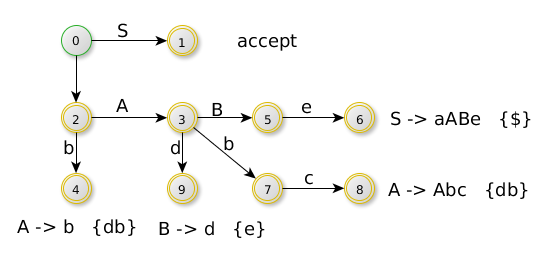
\includegraphics[scale=0.4]{Chapters/Img/c02_14.png}\\
\end{center} 

La sottolineatura significa che se arrivo in questo stato e sto leggendo come prossimo input una d o una b posso fare la riduzione della b usando A. Lo stesso vale per le altre, ovviamente con i loro simboli.
La roba fra parentesi graffe si chiama look-ahead set.

Nel grafo faccio quindi i seguenti passi (i numeri sono i nodi):
\begin{tabular}{ll}
    $0$   &   $abbcde\$$\\
    $0 \rightarrow 2$ consumando \lq $a$ \rq     &  $a || bbcde \$ $\\
    $2 \rightarrow 4$ consumando \lq $b$ \rq     &  $ab || bcde \$ $\\
    4 riduco $A \rightarrow b$  & $aA || bcde$\\
\end{tabular}
A questo punto torno al nodo 2 ovvero il precedente. Vado quindi in 3, perch\'e ho la A al posto della b che avevo prima.\\
torno a 2, vado in 3
\begin{tabular}{ll}
    $3 \rightarrow 7$ consumando \lq $b$ \rq     &  $aAb || cde \$ $\\
    $7 \rightarrow 8$ consumando \lq $c$ \rq     &  $aAbc || de \$ $\\
    8 riduco $A \rightarrow Abc$  & $aA || de$\\
    torno a 7, torno in 3, vado in 9 & \\
    $3 \rightarrow 9$ consumando \lq $d$ \rq     &  $aAd || e \$ $\\
    riduco $B \rightarrow d$ & $aAB || e \$ $\\
    torno a 3, vado in 5, vado in 6 & \\
    $5 \rightarrow 6$ consumando \lq $e$ \rq     &  $aABe || \$ $\\
    6 riduco $S \rightarrow aABe$ & $S || \$ $ \\
    torno a 0, vado in 1, ho finito & \\
\end{tabular}

Noi vogliamo avere grammatiche di tipo LALR(1). Grammatiche: $SLR(1) \subset LALR(1) \subset LR(1)$

\begin{center}
    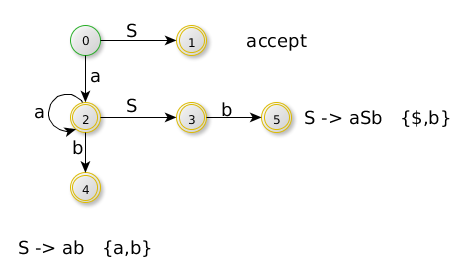
\includegraphics[scale=0.4]{Chapters/Img/c02_15.png}\\
\end{center} 

$S \rightarrow aSb | ab$\\
$w = aaabbb\$$

\begin{tabular}{ll}
    $0$                             &   $aaabbb\$$  \\ 
    $0 \rightarrow 2$               &   $a || aabbb\$$  \\ 
    $2 \rightarrow 2$               &   $aa || abbb\$$  \\ 
    $2 \rightarrow 2$               &   $aaa || bbb\$$  \\ 
    $2 \rightarrow 4$               &   $aaab || bb\$$  \\ 
    4 riduco $S \rightarrow ab$     &    $aaS || bb\$$  \\ 
    torno a 2, vado in 3, vado in 5 & \\
    $3 \rightarrow 5$               &   $aaSb || b\$$  \\ 
    5 riduco $S \rightarrow aSb$    &   $aS || b\$$  \\ 
    torno a 3, vado in 5            & \\
    $3 \rightarrow 5$               &   $aSb || \$$  \\ 
    5 riduco $S \rightarrow aSb$    &   $S || \$$  \\ 
    torno a 0, vado in 1, ho finito & \\
\end{tabular}

Questa \'e una tabella:
\begin{tabular}{|l|l|l|}
    \hline
            &   terminali $\cup \$$                                     &   $V \backslash T$     \\
    \hline
    stati   &   shift-k: leggi un simbolo di input e vai allo stato     &   goto-k: descrive le funzioni di transizione  \\
            &   reduce $A \rightarrow b $                               &   identificate dai non terminali quando consumi roba\\
    \hline
\end{tabular}

\section{Algoritmo di shift/reduce}
(comune a SLR(1), LR(1), LALR(1))

\begin{tabular}{ll}
    input   &   w, tabella di parsing bottom-up di tipo $\diamond$, con $\diamond$ scelto fra $\{SLR(1), LALR(1), LR(1)\}$ G.\\
    output  &   derivazione rightmost di w se $w \in L(G)$, altrimenti error()\\  
\end{tabular}

\begin{lstlisting}
    stack.push(s_0);
    buffer = w$;
    while(true){
        let s = stack.top();
        if(M[s,b] == shift-k){
            stack.push(b);
            stack.push(k);
            let b = buffer.readNext(); 
        } else if(M[s,b] == "reduce A -> beta"){
            stack.pop() 2|beta| simboli;
            let j tale che M[m, A] = gj;
            push(A);
            push(j);
            output "A -> beta";
        } else if(M[s,b] = accetta){
            break;
        } else {
            error();
        }
    }
\end{lstlisting}

*sketo*
$S \rightarrow aSb | ab $

\begin{center}
    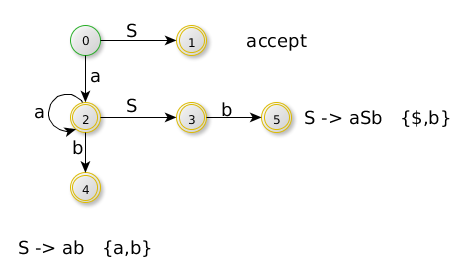
\includegraphics[scale=0.4]{Chapters/Img/c02_15.png}\\
\end{center} 

Questo \'e uguale ma scritto diversamente per separare $\{ \$, b\}$ in $\{4\}$ e $\{b\}$. Nel caso di $w=aaabbb\$$. Una caso rappresenta
il rao pi\'u in alto, mentre l'altro il secondo ramo (pi\'u interno).

\begin{center}
    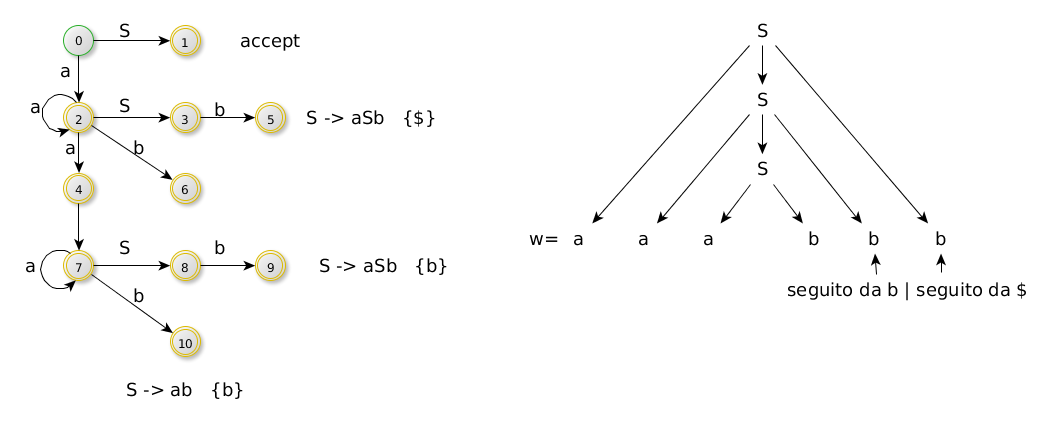
\includegraphics[scale=0.4]{Chapters/Img/c02_16.png}\\
\end{center} 

\begin{itemize}
    \item Automa caratteristico \\
    \item Lookahead Function \\
\end{itemize}

Coppie diverse di questi due insiemi ci danno tipi di grammatiche diverse.

Gli automi che stiamo utilizzando devono essere in grado di ricordare abbastanza da essere in grado di tornare indietro fino al punto 
in cui abbiamo sostituito una certa sequenza di terminali/non terminali con un'altra.

$G = (V,T,S,P)$, aggiungo una produzione $S' \rightarrow S$, $G' = (V \cup \{S'\},T,S',P \cup \{S' \rightarrow S\})$
$A \rightarrow \alpha . \beta $ 

All'inizio ho .S, ovvero non ho ancora letto nulla e devo leggere S.

All'inizio (il nodo iniziale), non ho ancora visto nulla. Visto che S pu\'o iniziare con aSb o ab non sappiamo davanti a quale sviluppo ci troviamo. Il primo stato \'e quindi 

$S' \rightarrow .S$\\
$S \rightarrow .aSb$\\
$S \rightarrow .ab$\\

Questo pu\'o essere visto come un nodo. Da questo stato mi muovo verso un altro stato (con una a-transizione, perch\'e vedo che iniziano 
quasi tutte con a). In questo stato avr\'o:
$S \rightarrow a.Sb$\\
$S \rightarrow a.b$\\

Adesso mi aspetto di vedere l'espansione di una S. Devo quindi aggiungere a questo nodo anche quelle produzioni, e diventa quindi:
$S \rightarrow a.Sb$\\
$S \rightarrow a.b$\\
$S \rightarrow .aSb$\\
$S \rightarrow .ab$\\

Notare che le ultime due sono le stesse delle ultime due del nodo prima. Quella \'e la chiusura, mentre le due prima sono i generatori dello stato (kernel dello stato, \textbf{kernel items}).

Gli stati che sono terminali (ovvero che nol disegno prima avevano le transizioni scritte vicino), sono del tipo $S \rightarrow ab.$ ,
ovvero che hanno incontrato di tutto e di cui si pu\'o eseguire la riduzione. Questi si chiamano \textbf{reducing items}.

Dallo stato con 4 items che avevo prima, si pu\'o fare una b-transizione che va in uno di quelli stati terminali, ovvero:
$S \rightarrow ab.$\\
Questo perch\'e la seconda produzione si aspetta b, che poi completa quello che viene generato da quella produzione.
Sempre da quello stato con 4 produzioni partir\'a anche una a-transizione ed una S-transizione. Per vedere che transizioni devo avere, 
devo vedere la prima lettera dopo il punto per ogni item di quel nodo.

\section{Items}
$G=(V,T,S,P)$\\
$G'=(V \cup \{ S' \},T,S',P \cup \{S' \rightarrow S\})$, con $S' \not\in V$.

Un LR(0)-item di G' \'e una produzione di G con un punto in qualche posizione del body, ovvero $A \rightarrow \alpha . \beta$ .
Alla produzione della forma $A \rightarrow \varepsilon$ corrisponde un solo LR(0)-item, ovvero $A \rightarrow . $\\
L'item $A \rightarrow \alpha . \beta $ \'e detto:
\begin{tabular}{ll}
    iniziale    &   se $A = S' \land \alpha = \varepsilon \land \beta = S$, cio\'e se l'item \'e $S' \rightarrow .S$\\
    accepting   &   se $A = S' \land \alpha = S \land \beta = \varepsilon $, cio\'e se l'item \'e $S' \rightarrow S.$\\
    kernel      &   se \'e un iniziale o tale che $\alpha != \varepsilon$ \\
    closure     &   se $\alpha = \varepsilon$ e non \'e iniziale \\
    reducing    &   se non \'e accepting e $\beta = \varepsilon$, cio\'e se il punto \'e in fondo $\land !accepting$ \\
\end{tabular}

\chapter{Bottom Up (Farina)}
Ricostruire, se $w \in L(G)$, una rightmost derivation al contrario
%%%%%%%%%%%%%%%%%%%%%%%%%%%%%%%%%%%%%%%%%%%%%%%%%%%%%%%%%%%%%%%%%%%%%%%%%%%%%%%%%%%%%%%%%%%%%%%%%%
\subsection{Esempio}
$S \rightarrow aABe$\\
$A \rightarrow Abc|b$\\
$B \rightarrow d$\\

w = abbcde visto che \'e rightmost devo espandere B dato che \'e il non terminale pi\'u a destra.
$S \rightarrow aABe \rightarrow aAde \rightarrow aAbcde \rightarrow abbcde $\\

\begin{center}
    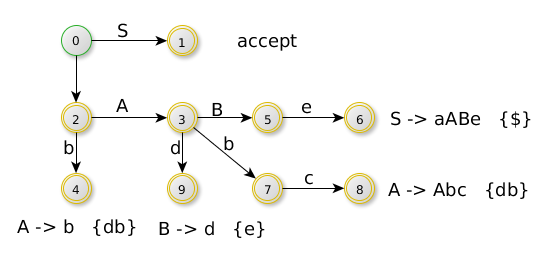
\includegraphics[scale=0.6]{Chapters/Img/c02_14.png}\\
\end{center} 

La sottolineatura significa che se arrivo in questo stato e sto leggendo come prossimo input una d o una b posso fare la riduzione della b usando A. Lo stesso vale per le altre, ovviamente con i loro simboli.
La roba fra parentesi graffe si chiama look-ahead set.

Nel grafo faccio quindi i seguenti passi (i numeri sono i nodi):
\begin{tabular}{ll}
    $0$   &   $abbcde\$$\\
    $0 \rightarrow 2$ consumando \lq $a$ \rq     &  $a || bbcde \$ $\\
    $2 \rightarrow 4$ consumando \lq $b$ \rq     &  $ab || bcde \$ $\\
    4 riduco $A \rightarrow b$  & $aA || bcde$\\
\end{tabular}
A questo punto torno al nodo 2 ovvero il precedente. Vado quindi in 3, perch\'e ho la A al posto della b che avevo prima.\\
torno a 2, vado in 3
\begin{tabular}{ll}
    $3 \rightarrow 7$ consumando \lq $b$ \rq     &  $aAb || cde \$ $\\
    $7 \rightarrow 8$ consumando \lq $c$ \rq     &  $aAbc || de \$ $\\
    8 riduco $A \rightarrow Abc$  & $aA || de$\\
    torno a 7, torno in 3, vado in 9 & \\
    $3 \rightarrow 9$ consumando \lq $d$ \rq     &  $aAd || e \$ $\\
    riduco $B \rightarrow d$ & $aAB || e \$ $\\
    torno a 3, vado in 5, vado in 6 & \\
    $5 \rightarrow 6$ consumando \lq $e$ \rq     &  $aABe || \$ $\\
    6 riduco $S \rightarrow aABe$ & $S || \$ $ \\
    torno a 0, vado in 1, ho finito & \\
\end{tabular}

Noi vogliamo avere grammatiche di tipo LALR(1). Grammatiche: $SLR(1) \subset LALR(1) \subset LR(1)$

\begin{center}
    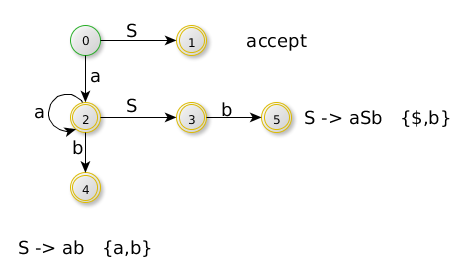
\includegraphics[scale=0.6]{Chapters/Img/c02_15.png}\\
\end{center} 

$S \rightarrow aSb | ab$\\
$w = aaabbb\$$

\begin{tabular}{ll}
    $0$                             &   $aaabbb\$$  \\ 
    $0 \rightarrow 2$               &   $a || aabbb\$$  \\ 
    $2 \rightarrow 2$               &   $aa || abbb\$$  \\ 
    $2 \rightarrow 2$               &   $aaa || bbb\$$  \\ 
    $2 \rightarrow 4$               &   $aaab || bb\$$  \\ 
    4 riduco $S \rightarrow ab$     &    $aaS || bb\$$  \\ 
    torno a 2, vado in 3, vado in 5 & \\
    $3 \rightarrow 5$               &   $aaSb || b\$$  \\ 
    5 riduco $S \rightarrow aSb$    &   $aS || b\$$  \\ 
    torno a 3, vado in 5            & \\
    $3 \rightarrow 5$               &   $aSb || \$$  \\ 
    5 riduco $S \rightarrow aSb$    &   $S || \$$  \\ 
    torno a 0, vado in 1, ho finito & \\
\end{tabular}\\[5pt]

Questa \'e una tabella:\\
\begin{tabular}{|l|l|l|}
    \hline
            &   terminali $\cup\ \$$                                     &   $V \backslash T$     \\
    \hline
    stati   &   shift-k: leggi un simbolo di input e vai allo stato     &   goto-k: descrive le funzioni di transizione  \\
            &   reduce $A \rightarrow b $                               &   identificate dai non terminali quando consumi roba\\
    \hline
\end{tabular}

\section{Algoritmo di shift/reduce}
(comune a SLR(1), LR(1), LALR(1))

\begin{tabular}{ll}
    input   &   w, tabella di parsing bottom-up di tipo $\diamond$, con $\diamond$ scelto fra $\{SLR(1), LALR(1), LR(1)\}$ G.\\
    output  &   derivazione rightmost di w se $w \in L(G)$, altrimenti error()\\  
\end{tabular}

\begin{lstlisting}
    stack.push(s_0);
    buffer = w$;
    while(true){
        let s = stack.top();
        if(M[s,b] == shift-k){
            stack.push(b);
            stack.push(k);
            let b = buffer.readNext(); 
        } else if(M[s,b] == "reduce A -> beta"){
            stack.pop() 2|beta| simboli;
            let j tale che M[m, A] = gj;
            push(A);
            push(j);
            output "A -> beta";
        } else if(M[s,b] = accetta){
            break;
        } else {
            error();
        }
    }
\end{lstlisting}

*sketo*
$S \rightarrow aSb | ab $

\begin{center}
    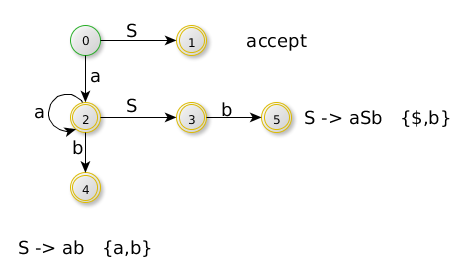
\includegraphics[scale=0.6]{Chapters/Img/c02_15.png}\\
\end{center} 

Questo \'e uguale ma scritto diversamente per separare $\{ \$, b\}$ in $\{4\}$ e $\{b\}$. Nel caso di $w=aaabbb\$$. Una caso rappresenta
il ramo pi\'u in alto, mentre l'altro il secondo ramo (pi\'u interno).

\begin{center}
    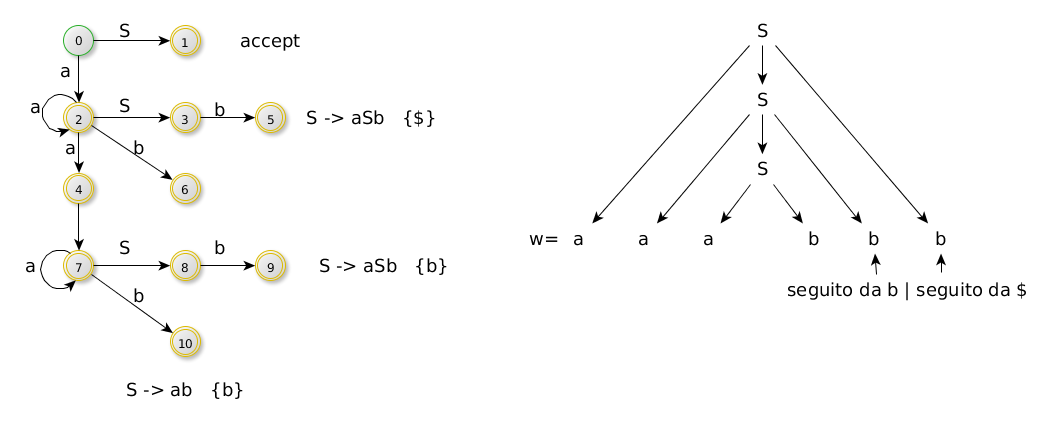
\includegraphics[scale=0.45]{Chapters/Img/c02_16.png}\\
\end{center} 

\begin{itemize}
    \item Automa caratteristico \\
    \item Lookahead Function \\
\end{itemize}

Coppie diverse di questi due insiemi ci danno tipi di grammatiche diverse.

Gli automi che stiamo utilizzando devono essere in grado di ricordare abbastanza da essere in grado di tornare indietro fino al punto 
in cui abbiamo sostituito una certa sequenza di terminali/non terminali con un'altra.

$G = (V,T,S,P)$, aggiungo una produzione $S' \rightarrow S \implies G' = (V \cup \{S'\},T,S',P \cup \{S' \rightarrow S\})$\\
\subsection{Closure}

All'inizio ho .S, ovvero non ho ancora letto nulla e devo leggere S.

All'inizio (il nodo iniziale), non ho ancora visto nulla. Visto che S pu\'o iniziare con aSb o ab non sappiamo davanti a quale sviluppo ci troviamo. Il primo stato \'e quindi 

$S' \rightarrow .S$\\
$S \rightarrow .aSb$\\
$S \rightarrow .ab$\\

Questo pu\'o essere visto come un nodo. Da questo stato mi muovo verso un altro stato (con una a-transizione, perch\'e vedo che iniziano 
quasi tutte con a). In questo stato avr\'o:
$S \rightarrow a.Sb$\\
$S \rightarrow a.b$\\

Adesso mi aspetto di vedere l'espansione di una S. Devo quindi aggiungere a questo nodo anche quelle produzioni, e diventa quindi:
$S \rightarrow a.Sb$\\
$S \rightarrow a.b$\\
$S \rightarrow .aSb$\\
$S \rightarrow .ab$\\

Quando computo uno stato ho i \textbf{kernel items} che poi vengono espansi con la \textbf{closure}.
Notare che gli ultimi due items sono gli stessi degli ultimi due del nodo precedente. 
Quella \'e la chiusura, mentre i primi due sono i generatori dello stato (kernel dello stato o \textbf{kernel items}).

Gli stati che terminali dell'automa (le foglie) sono del tipo $S \rightarrow ab.$ ,
quindi hanno incontrato tutto i simboli e possono essere ridotti (\textbf{reducing items}).

Dallo stato con 4 items che avevo prima, si pu\'o fare una b-transizione che va in uno di quelli stati terminali, ovvero:
$S \rightarrow ab.$\\
Questo perch\'e la seconda produzione si aspetta b, che poi completa quello che viene generato da quella produzione.
Sempre da quello stato con 4 produzioni partir\'a anche una a-transizione ed una S-transizione. Per vedere che transizioni devo avere, 
devo vedere la prima lettera dopo il punto per ogni item di quel nodo.

\section{Items}
$G=(V,T,S,P)$\\
$G'=(V \cup \{ S' \},T,S',P \cup \{S' \rightarrow S\})$, con $S' \not\in V$.

Un LR(0)-item di G' \'e una produzione di G con un punto in qualche posizione del body, ovvero $A \rightarrow \alpha . \beta$ .
Alla produzione della forma $A \rightarrow \varepsilon$ corrisponde un solo LR(0)-item, ovvero $A \rightarrow . $\\
L'item $A \rightarrow \alpha . \beta $ \'e detto:
\begin{tabular}{ll}
    iniziale    &   se $A = S' \land \alpha = \varepsilon \land \beta = S$, cio\'e se l'item \'e $S' \rightarrow .S$\\
    accepting   &   se $A = S' \land \alpha = S \land \beta = \varepsilon $, cio\'e se l'item \'e $S' \rightarrow S.$\\
    kernel      &   se \'e un iniziale o tale che $\alpha != \varepsilon$ \\
    closure     &   se $\alpha = \varepsilon$ e non \'e iniziale \\
    reducing    &   se non \'e accepting e $\beta = \varepsilon$, cio\'e se il punto \'e in fondo $\land !accepting$ \\
\end{tabular}


\chapter{Costruzione di un automa caratteristico LR(0) o LR(1)}
(data un'appropriata istanziazione di $P_0$ (stato iniziale) e closure function)

Prima di tutto facciamo la costruzione dell'automa caratteristico, usando l'algoritmo sotto riportato.

Istanziando $P_0$, closure otteniamo:
\begin{itemize}
	\item automi caratteristici LR(0)-automi $\leftarrow$ parsing SLR(1)\\
	\item automi caratteristici LR(1)-automi $\leftarrow$ parsing LR(1)\\
\end{itemize}
Lookahead function $LA:(FxP) \rightarrow p(T \cup \{ \$ \} )$
con F = insieme degli stati finali dell'automa caratteristico considerato. Si considerano stati finali gli stati che contengono almeno un reducing item.

L'automa caratteristico sar\'a necessario per la creazione della tabella di parsing.

\begin{lstlisting}
	Inizializzare la collezione Q di stati come {P_0};
	flag P_0 come non-marcato;

	while(ho uno stato non marcato P in Q){
		marca P;
		foreach(A -> a.Ybeta in P){
			tmp.add( A->aY.beta );
		}
		if(tmp == kernel(R)){ //per qualche R in Q
			tau(P, Y) = R; //goto function
		} else {
			newState = closure(tmp);
			tau(P, Y) = newState;
			Q.add(newState); //come non-marcato 
		}
	}
\end{lstlisting}

\subsection{Esempi di closure, grammatica SLR}
se ho la grammatica:\\
$S' \rightarrow S$\\
$S \rightarrow aSb|ab$\\
$closure_0(\{ S' \rightarrow .S\})$ \'e composta da:\\
$S \rightarrow .aSb$\\
$S \rightarrow .ab$\\

Se invece ho una grammatica:\\ 
$E' \rightarrow E$\\
$E \rightarrow E + T | T$\\
$T \rightarrow T * F | F$\\
$F \rightarrow (E) | id $\\

Allora $closure_0(\{ E' \rightarrow .E \})$ diventa \\
$E \rightarrow .E + T $ quelle con il punto prima della E le ho gi\'a aggiunte, non faccio nulla\\
$E \rightarrow .T $ ora aggiungo quelle con il punto prima della T\\
$T \rightarrow .T * F $ quelle con il punto prima della T le ho gi\'a aggiunte, non faccio nulla\\
$T \rightarrow .F $ ora aggiungo quelle con il punto prima della F\\
$F \rightarrow .(E)$ terminale dopo il punto, non devo aggiungere nulla\\
$F \rightarrow .id$ terminale dopo il punto, non devo aggiungere nulla\\
Si devono fare in ordine per non dimenticarsene in giro.

%%%%%%%%%%%%%%%%%%%%%%%%%%%%%%%%%%%%%%%%%%%%%%%%%%%%%%%%%%%%%%%%%%%%%%%%%%%%%%%%%%%%%%%%%%%%%%%%%%%%%%%%%%%%%%%%%%%%%%%%%%%%%%%%%%%%
\section{Algoritmo di $closure_0(P)$}
\begin{lstlisting}
	tag ogni item in P come non-marcato

	while(ho ancora un item I non marcato in P){
		marca I;
		if(I ha la forma A -> alpha .B beta){
			foreach ((B -> Y) in P){
				if(B -> Y not in P){
					add(B -> .Ya);
					segna P come non-marcato;
				}
			}
		}
	}
	return P;
\end{lstlisting}

\section{LR(0) automaton}
Si ricava utilizzando, nell'algoritmo di costruzione dell'automa caratteristico:
\begin{itemize}
	\item $P_0 = closure_0 ( \{ S' \rightarrow .S \} )$ per la grammatica G arricchita con $S' \rightarrow S$\\
	\item $ closure_0 $ per closure\\
\end{itemize}

%%%%%%%%%%%%%%%%%%%%%%%%%%%%%%%%%%%%%%%%%%%%%%%%%%%%%%%%%%%%%%%%%%%%%%%%%%%%%%%%%%%%%%%%%%%%%%%%%%%%%%%%%%%%%%%%%%%%%%%%%%%%%%%%%%%%
\subsection{Esempio}
$ S' \rightarrow S $\\
$ S \rightarrow aSb | ab $\\

\begin{tabular}{lll}
	$P_0=$ 	&	$S' \rightarrow .S$ 	& \\
			&	$S \rightarrow .aSb$ 	& \\
		 	&	$S \rightarrow .ab$ 	& \\
	$P_1=$ 	&	$S' \rightarrow S.$ 	& ci si arriva con una S-transizione (ACCEPT)\\
	$P_2=$ 	&	$S \rightarrow a.Sb$ 	& ci si arriva con una a-transizione\\
			&	$S \rightarrow a.b$ 	& \\
		 	&	$S \rightarrow .aSb$ 	& \\
		 	&	$S \rightarrow .ab$ 	& \\
		 	& 	$P_0 \text{ e } P_1$ sono finiti, guardo $P_2$ & \\
	$P_3=$ 	&	$S \rightarrow aS.b$ 	& ci si arriva con una S-transizione da $P_2$\\
	$P_4=$ 	&	$S \rightarrow ab.$ 	& ci si arriva con una b-transizione da $P_2$\\
	$P_5=$ 	&	$S \rightarrow .aSb$ 	& ci si arriva con una a-transizione da $P_2$ (stesse righe di $P_2$)\\
		 	&	$S \rightarrow .ab$ 	& la freccia quindi va da $P_2$ a $P_2$, perch\'e $P_5 \subset P_2$\\
		 	&	ora guardo $P_3$	& \\
	$P_6=$ 	&	$S \rightarrow aSb.$ 	& ci si arriva con una b-transizione da $P_3$\\
\end{tabular}  

%%%%%%%%%%%%%%%%%%%%%%%%%%%%%%%%%%%%%%%%%%%%%%%%%%%%%%%%%%%%%%%%%%%%%%%%%%%%%%%%%%%%%%%%%%%%%%%%%%%%%%%%%%%%%%%%%%%%%%%%%%%%%%%%%%%%
\section{Creazione della tabella di parsing}

\begin{tabular}{ll}
	$\tau$ 		&	funzione di transizione (GOTO) dell'automa caratteristico considerato.\\
	\textbf{LA} 	& 	lookahead function considerata.\\
\end{tabular}

La tabella di parsing bottom-up per la coppia prescelta di automa e lookahead function \'e una matrice 
$Q \otimes (V \cup \{ \$ \})$ dove Q \'e l'insieme degli stati dell'automa prescelto. \\[10pt]

$\forall$ entry (P,Y):
\begin{tabular}{ll}
	inserire \textbf{shift}					&	se $Y \in T \land \tau(P,Y) = R $\\
	inserire \textbf{reduce} $A \rightarrow \beta$   &	se $A \rightarrow \beta . \in P \land Y \in LA(P, A \rightarrow \beta) $\\
	inserire \textbf{accept()}				&	se $Y = \$ \land S' \rightarrow S. \in P $\\
	inserire \textbf{error()}				&	se $Y \in T \cup \{\$\} \land$ non \'e ancora stato inserito nulla\\
	applicando i passi precedenti 			& \\
	inserire \textbf{goto R}  				&	se $Y \in V\backslash T \land \tau (P,Y) = R $\\
\end{tabular}

%%%%%%%%%%%%%%%%%%%%%%%%%%%%%%%%%%%%%%%%%%%%%%%%%%%%%%%%%%%%%%%%%%%%%%%%%%%%%%%%%%%%%%%%%%%%%%%%%%%%%%%%%%%%%%%%%%%%%%%%%%%%%%%%%%%%
\subsection{Esercizio}
$SLR(1)$\\
$LR(0)$ automa \\
$LA(P, A \rightarrow \beta) = follow(A)\ \forall\ P \in Q$ (automa)\\



\begin{tabular}{|c|c|c|c|c|}
	\hline
	[numero nodo] 	&  [parte che & pu\'o avere & conflitti] & [goto part]\\
	\hline
		& 	\textbf{a} 	&	\textbf{b} 	& 	$\bm{\$}$ 	&	\textbf{S} 	\\
	\hline
	\textbf{0} 	&	S2	&		&			&	g1	\\
	\hline
	\textbf{1} 	&		&		&	ACCEPT	&		\\
	\hline
	\textbf{2} 	&	S2	&	S4	&			&	g3	\\
	\hline
	\textbf{3} 	&		&	s5	&			&		\\
	\hline
	\textbf{4} 	&		&	$R: S\rightarrow ab $	&	$R: S\rightarrow ab $		&		\\
	\hline
	\textbf{5} 	&		&	$R: S\rightarrow aSb $	&	$R: S\rightarrow aSb $		&		\\
	\hline
\end{tabular}

S = shift
R = reduce
g = goto

Se ho la parola $w = aabb\$$ faccio:
\begin{tabular}{|lll|}
	\hline
	0 			& 	$aabb\$$ 	& 	sono in 0 e vedo a. Faccio [0, a] nella tabella \\
	0a2			& 	$abb\$$ 	& 	sono in 2 e vedo a. Faccio [2, a] nella tabella \\
	0a2a2		& 	$bb\$$ 		& 	sono in 2 e vedo b. Faccio [2, b] nella tabella \\
	aa2a2b4 	& 	$b\$$ 		& 	sono in 4 e vedo b. Faccio il reduce (cella 4b) \\
				&				&	visto che crea 2S, e [2, S] = g3, aggiungo 3 	\\
	0a2S3		& 	$b\$$ 		& 	sono in 3 e vedo b. Faccio [3, b] nella tabella \\
	0a2S3b5		& 	$\$$ 		& 	sono in 5 e vedo $\$$. Faccio il reduce (cella 5$\$$ \\
				&				&	visto che crea 0S, e [0, S] = g1, aggiungo 1 	\\
	0S1			& 	$\$$ 		& 	ok perch\'e [S, 1] \'e accept 					\\
	\hline
\end{tabular}

\subsection{Esempio Conflitti Shift/Reduce}
(Esempio con una grammatica ambigua)\\

$E \rightarrow E + E | E * E | id $\\
automa LR(0)

\begin{center}
    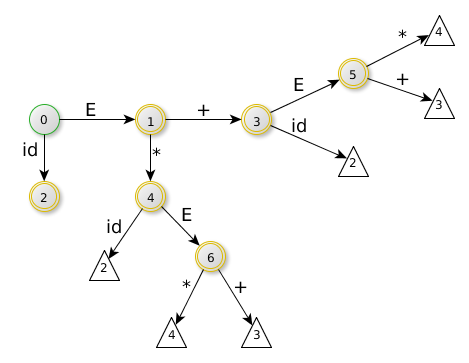
\includegraphics[scale=0.6]{Chapters/Img/c02_17.png}\\
\end{center} 

//Se va a triangoli, non parte dal kernel, altrimenti si(?)

0 =
\begin{tabular}{l}
	$E' \rightarrow .E$		\\
	$E \rightarrow .E + E$	\\
	$E \rightarrow .E * E$	\\
	$E \rightarrow .id$		\\
\end{tabular}\\[5pt]

1 =
\begin{tabular}{l}
	$E' \rightarrow E.$		\\
	$E \rightarrow E. + E$	\\
	$E \rightarrow E. * E$	\\
\end{tabular}\\[5pt]

2 =
\begin{tabular}{l}
	$E \rightarrow id.$		\\
\end{tabular}\\[5pt]

3 =
\begin{tabular}{l}
	$E \rightarrow E + .E$		\\
	$E \rightarrow .E * E$		\\
	$E \rightarrow .id $		\\
\end{tabular}\\[5pt]

4 =
\begin{tabular}{l}
	$E \rightarrow E * .E$		\\
	$E \rightarrow .E + E$		\\
	$E \rightarrow .E * E$		\\
	$E \rightarrow .id $		\\
\end{tabular}\\[5pt]

5 =
\begin{tabular}{l}
	$E \rightarrow E + E.$		\\
	$E \rightarrow E. + E$		\\
	$E \rightarrow E. * E$		\\
\end{tabular}\\[5pt]

6 =
\begin{tabular}{l}
	$E \rightarrow E * E.$		\\
	$E \rightarrow E. + E$		\\
	$E \rightarrow E. * E$		\\
\end{tabular}\\[5pt]

\begin{tabular}{|c|c|c|c|c|}
	\hline
		&	\textbf{id} 		&	$\bm{+}$	&	$\bm{*}$	&	$\bm{\$} $	\\
	\hline
	\textbf{0}	&	S2 		&		&		&			\\	
	\hline
	\textbf{1}	&	 		&	S3	&	S4	&	ACCEPT	\\	
	\hline
	\textbf{2}	&	 		&	$R:\ E \rightarrow id $		&	$R:\ E \rightarrow id $	& $R:\ E \rightarrow id $	\\	
	\hline
	\textbf{3}	&	S2 		&		&		&			\\	
	\hline
	\textbf{4}	&	S2 		&		&		&			\\	
	\hline
	\textbf{5}	&	 		&	$\bm{S3,\ R:\ E \rightarrow E+E}$	&	$\bm{S4,\ R:\ E \rightarrow E+E}$	&	$R:\ E \rightarrow E+E$		\\	
	\hline
	\textbf{6}	&	 		&	$\bm{S3,\ R:\ E \rightarrow E*E}$	&	$\bm{S4,\ R:\ E \rightarrow E*E}$	&	$R:\ E \rightarrow E*E$		\\	
	\hline
\end{tabular}\\[5pt]

\begin{tcolorbox}\begin{center}
	Visto che ci sono \textbf{conflitti} nella tabella, questa grammatica \textbf{non \'e SLR}. 
\end{center}\end{tcolorbox}

In questo caso i conflitti sono di tipo Shift/Reduce.
Ma possono essere anche di tipo Reduce/Reduce.

Tra le produzioni nelle celle colorate, quali sono quelle da tenere per avere una grammatica che associa a sinistra?

Nella cella [5, +] devo tenere R \lq\lq $E \rightarrow E + E $ \rq\rq\\
Nella cella [5, *] devo tenereS4 \\
Nella cella [6, +] devo tenere R \lq\lq $E \rightarrow E * E $ \rq\rq\\
Nella cella [6, *] devo tenere R \lq\lq $E \rightarrow E * E $ \rq\rq\\  

$W = id * id + id \$ $\\
$ 0 $\\
$ 0id2 $\\
$ 0E1 $\\
$ 0E1*4id2 $\\
$ 0E1*4E6 $\\
$ 0E1 $\\
$ 0E1+3id2 $\\
$ 0E1+3E5 $\\
$ 0E1 $\\
$ ok $\\

\Tree[.E [.E [.E id ] * [.E id ] ] + [.E id ] ]

\subsection{Esempio Conflitti Reduce/Reduce}
$S \rightarrow aAd | bBd | aBe | bAe$\\
$A \rightarrow c $\\
$B \rightarrow c $\\

Questa grammatica produce 4 stringhe, ogniuna in un modo, e quindi ovviamente non \'e ambigua.

\begin{center}
    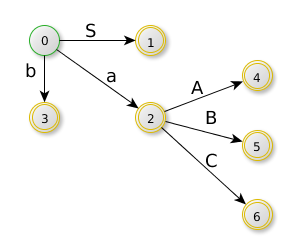
\includegraphics[scale=0.6]{Chapters/Img/c02_18.png}\\
\end{center} 

0 =
\begin{tabular}{l}
	$S' \rightarrow .S $		\\
	$S  \rightarrow .aAd $		\\
	$S  \rightarrow .bBd $		\\
	$S  \rightarrow .aBe $		\\
	$S  \rightarrow .bAe $		\\
\end{tabular}\\[5pt]

1 =
\begin{tabular}{l}
	$S' \rightarrow S. $		\\
\end{tabular}\\[5pt]

2 =
\begin{tabular}{l}
	$S \rightarrow a.Ad  $		\\
	$S  \rightarrow a.Be $		\\
	$A  \rightarrow .c $		\\
	$B  \rightarrow .c $		\\
\end{tabular}\\[5pt]

3 =
\begin{tabular}{l}
	$S \rightarrow b.Bd  $		\\
	$S  \rightarrow b.Ae $		\\
	$B  \rightarrow .c $		\\
	$A  \rightarrow .c $		\\
\end{tabular}\\[5pt]

4 =
\begin{tabular}{l}
	$S \rightarrow aA.d $		\\
\end{tabular}\\[5pt]

5 =
\begin{tabular}{l}
	$S \rightarrow aB.e $		\\
\end{tabular}\\[5pt]

6 =
\begin{tabular}{l}
	$A \rightarrow c. $		\\
	$B \rightarrow c. $		\\
\end{tabular}\\[5pt]

\begin{tabular}{|c|c|c|c|c|c|}
	\hline
		&	a 	& 	b 	&	d 	& 	e 	&	$\$$ 	\\
	\hline
	6	&	 	& 	& 	$R:\ A \rightarrow c $ 	&	$R:\ A \rightarrow c $ 	& 	\\	
		&	 	& 	& 	$R:\ B \rightarrow c $ 	&	$R:\ B \rightarrow c $ 	& 	\\	
	\hline
\end{tabular}

Anche se non \'e una grammatica ambigua ci sono multiple entries. Questo dipende dal modo in cui scegliamo i follow. 
Nel parsing canonico infatti non si usano gli item LR(0) ma gli item LR(1) perch\'e ci portiamo dietro informazione direttamente
dagli item. Questo riduce/rimuove i problemi di questo tipo.

Un item LR(1) canonico \'e del tipo $A \rightarrow \alpha . \beta, \delta$ con $\delta \subset T \cup \{ \$ \}$.\\

\section{LR(1)}
Negli automi caratteristici LR(1) si considera come stato iniziale lo stato che si ottiene facendo: 
$closure_1 (\{[ S' \rightarrow .S, \{ \$\}  ]\})$

\subsection{Esempio grammatica LR(1)}
$S \rightarrow aAd | aBe | bBd |bAe $\\
$A \rightarrow c$\\
$B \rightarrow c$\\


\begin{center}
    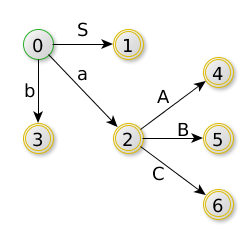
\includegraphics[scale=0.6]{Chapters/Img/c05_01.png}\\
\end{center}

0 =
\begin{tabular}{l}
	$S' \rightarrow .S,\ 	\{ \$ \} $		\\
	$S \rightarrow .aAd,\ 	\{ \$ \} $		\\
	$S \rightarrow .aBe,\ 	\{ \$ \} $		\\
	$S \rightarrow .bBd,\ 	\{ \$ \} $		\\
	$S \rightarrow .bAe,\ 	\{ \$ \} $		\\
\end{tabular}\\[5pt]

1 =
\begin{tabular}{l}
	$S' \rightarrow S.,\ 	\{ \$ \} $		\\
\end{tabular}\\[5pt]

2 =
\begin{tabular}{l}
	$S \rightarrow a.Ad,\ 	\{ \$ \} $		\\
	$S \rightarrow a.Be,\ 	\{ \$ \} $		\\
	$A \rightarrow .c,\ 	\{ d \} $		\\
	$B \rightarrow .c,\ 	\{ e \} $		\\
\end{tabular}\\[5pt]


3 =
\begin{tabular}{l}
	$S \rightarrow b.Bd,\ 	\{ ? \} $		\\
	$S \rightarrow b.Ae,\ 	\{ ? \} $		\\
	$A \rightarrow .c,\ 	\{ ?\} $		\\
	$B \rightarrow .c,\ 	\{ ?\} $		\\
\end{tabular}\\[5pt]


4 =
\begin{tabular}{l}
	$S \rightarrow aA.d,\ 	\{ ? \} $		\\
\end{tabular}\\[5pt]

5 =
\begin{tabular}{l}
	$S \rightarrow aB.e,\ 	\{ ? \} $		\\
\end{tabular}\\[5pt]

6 =
\begin{tabular}{l}
	$A \rightarrow c.,\ 	\{ d \} $		\\
	$B \rightarrow c.,\ 	\{ e \} $		\\
\end{tabular}\\[5pt]

\section{Algoritmo $Closure_1(P)$}
\begin{lstlisting}
	every item in P is unmarked
	while(exists an item I in P unmarked){
		mark I;
		if([ A -> alpha. B beta, delta ] in I){
			delta1 = Union(d in delta) first(beta d)
			foreach([ B -> Y ] in P){
				if([ B -> .Y ] not in proj(P)){ //projection is the first component of an item yet collected
					P.add([ B -> .Y, delta1] as unmarked)
				} else {
					if([ B -> .Y, gamma ] in P && delta1 not subset gamma ){
						update [ B -> .Y, gamma ] in [Bb -> .Y, gamma U delta1] as unmarked;
					}
				}
			}
		}
	}
	return P;
\end{lstlisting}

\section{Esempio grammatica LALR}

$S \rightarrow L = R | R$\\
$L \rightarrow *R|id$\\
$R \rightarrow L$\\

Computare la $closure_1( \{ [ S' \rightarrow S,\ \{\$\} ] \} )$ (nodo 0 e disegnare l'automa LR(1). Capire se \'e SLR(1)).

\begin{center}
    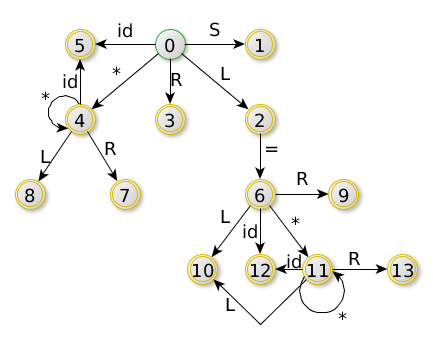
\includegraphics[scale=0.6]{Chapters/Img/c05_02.png}\\
\end{center}

0 =
\begin{tabular}{l}
	$S' \rightarrow .S,\ 	\{ \$ \} $		\\
	$S \rightarrow .L = R,\ 	\{ \$ \} $		\\
	$S \rightarrow .R,\ 	\{ \$ \} $		\\
	$L \rightarrow .*R,\ 	\{ \$ \} $		\\
	$L \rightarrow .id,\ 	\{ \$ \} $		\\
	$R \rightarrow .L,\ 	\{ \$ \} $		\\
\end{tabular}\\[5pt]

1 =
\begin{tabular}{l}
	$S' \rightarrow S.,\ 	\{ \$ \} $		\\
\end{tabular}\\[5pt]

2 =
\begin{tabular}{l}
	$S \rightarrow L.=R,\ 	\{ \$ \} $		\\
	$R \rightarrow L.,\ 	\{ \$ \} $		\\
\end{tabular}\\[5pt]

3 =
\begin{tabular}{l}
	$S \rightarrow R.,\ 	\{ \$ \} $		\\
\end{tabular}\\[5pt]

4 =
\begin{tabular}{l}
	$L \rightarrow *.R,\ 	\{ =, \$ \} $		\\
	$R \rightarrow .L,\ 	\{ =, \$ \} $		\\
	$L \rightarrow .id,\ 	\{ =, \$ \} $		\\
	$L \rightarrow .*R,\ 	\{ =, \$ \} $		\\
\end{tabular}\\[5pt]

5 =
\begin{tabular}{l}
	$L \rightarrow id.,\ 	\{ =, \$ \} $		\\
\end{tabular}\\[5pt]

6 =
\begin{tabular}{l}
	$S \rightarrow L = .R,\ 	\{ \$ \} $		\\
	$R \rightarrow .L,\ 	\{ \$ \} $		\\
	$L \rightarrow .*R,\ 	\{ \$ \} $		\\
	$L \rightarrow .id,\ 	\{ \$ \} $		\\
\end{tabular}\\[5pt]

7 =
\begin{tabular}{l}
	$L \rightarrow *R.,\ 	\{ =, \$ \} $		\\
\end{tabular}\\[5pt]

8 =
\begin{tabular}{l}
	$R \rightarrow L.,\ 	\{ =, \$ \} $		\\
\end{tabular}\\[5pt]

9 =
\begin{tabular}{l}
	$S \rightarrow L = R.,\ 	\{ \$ \} $		\\
\end{tabular}\\[5pt]

10 =
\begin{tabular}{l}
	$R \rightarrow L.,\ 	\{ \$ \} $		\\
\end{tabular}\\[5pt]

11 =
\begin{tabular}{l}
	$L \rightarrow *.R,\ 	\{ \$ \} $		\\
	$R \rightarrow .L,\ 	\{ \$ \} $		\\
	$L \rightarrow .*R,\ 	\{ \$ \} $		\\
	$L \rightarrow .id,\ 	\{ \$ \} $		\\
\end{tabular}\\[5pt]

12 =
\begin{tabular}{l}
	$L \rightarrow id.,\ 	\{ \$ \} $		\\
\end{tabular}\\[5pt]

13 =
\begin{tabular}{l}
	$L \rightarrow *R.,\ 	\{ \$ \} $		\\
\end{tabular}\\[5pt]

Notare che i nodi 8 e 10 sembrano uguali ma non lo sono perch\'e hanno lookahead diversi; anche nel gravo saranno nodi distinti 
mentre se avessimo fatto un automa LR(0) sarebbero stati uniti. Lo stesso automa LR(0):

\begin{center}
    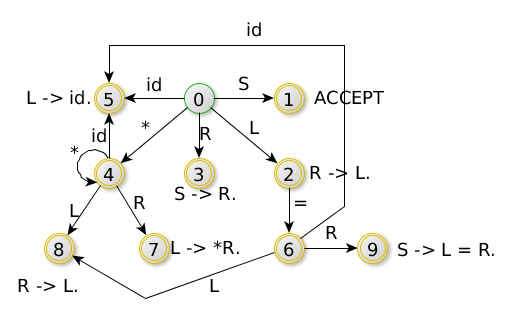
\includegraphics[scale=0.6]{Chapters/Img/c05_03.png}\\
\end{center}

Quest'ultimo automa ha almeno uno shift/reduce conflict mentre l'automa LR(1) non ne avr\'a.

Guardiamo se \'e SLR(1) 

\begin{tabular}{|c|c|c|c|c|c|c|c|}
	\hline
		&	\textbf{id} 	& $\bm{*}$	& $\bm{*}$	& $\bm{*}$	& 	\textbf{S}  & \textbf{L} & \textbf{R} \\  
	\hline
	\textbf{0}	&	S5 	& S4 	& 		& 		& 1 	& 2 	& 3 	\\
	\hline
	\textbf{1}	&		& 		& 		& ACC 	& 		& 		& 		\\
	\hline
	\textbf{2}	&		& 		& S6 	& r: $R \rightarrow L$ & 	& 	 	& 		\\
	\hline
	\textbf{3}	&		& 		& 		& r: $S \rightarrow R$ & 	& 		& 		\\
	\hline
	\textbf{4}	&	S5 & S4 	& 		& 						&	& 8 	& 7		\\
	\hline
	\textbf{5}	&		&		& r: $L \rightarrow id$ & r: $L \rightarrow id$ & 	&	&	\\
	\hline
	\textbf{6}	&	S12 & S11 	& 		& 						&	& 10 	& 9		\\	
	\hline
	\textbf{7}	&		&		& r: $L \rightarrow *R$ & r: $L \rightarrow *R$ & 	&	&	\\
	\hline
	\textbf{8}	&		&		& r: $R \rightarrow L$ & r: $R \rightarrow L$  & 	&	&	\\	
	\hline
	\textbf{9}	&		& 		& 		& r: $S \rightarrow L = R$ & 	& 		& 		\\	
	\hline
	\textbf{10}	&		& 		& 		& r: $R \rightarrow L$ & 	& 		& 		\\	
	\hline
	\textbf{11}	&	S12 & S11 	& 		& 						&	& 10 	& 13		\\		
	\hline
	\textbf{12}	&		& 		& 		& r: $L \rightarrow id$ & 	& 		& 		\\		
	\hline
	\textbf{13}	&		& 		& 		& r: $L \rightarrow *R$ & 	& 		& 		\\		
	\hline
\end{tabular}

visto che non ci sono conglitti questa grammatica \'e LR(1).
Gli stati 4 e 11 hanno la stessa proiezione; possiamo quindi fare: 
$P_1 \cup P_2\quad A \rightarrow \alpha . \beta,\ \delta_1 \cup \delta_2$.

Lo posso fare per 4 e 11, 5 e 12, 8 e 10, 7 e 13

\begin{tabular}{|c|c|c|c|c|c|c|c|}
	\hline
		&	\textbf{id} 	& $\bm{*}$	& $\bm{*}$	& $\bm{*}$	& 	\textbf{S}  & \textbf{L} & \textbf{R} \\  
	\hline
	\textbf{411}	&	S512 & S411 	& 		& 		& 810 	& 2 	& 713 	\\
	\hline
	\textbf{512}	&		& 		& r: $L \rightarrow id$		& r: $L \rightarrow id$ 	& 		& 		& 		\\
	\hline
	\textbf{713}	&		& 		& r: $L \rightarrow *R$ 	& r: $L \rightarrow *R$		& 		& 	 	& 		\\
	\hline
	\textbf{810}	&		& 		& r: $r \rightarrow L$ 	& r: $R \rightarrow L$		& 		& 	 	& 		\\
	\hline
\end{tabular}

Dovr\'o anche aggiornare i vari shift e goto delle altre righe per farli andare ai nodi nuovi. S5 ed S12 diventeranno S512.

La grammatica cos'\i generata \'e LALR perch\'e nella tabella non ci sono conflitti.

\subsection{Ricorda}
$ SLR(1) \subset LALR(1) \subset LR(1)$

Grammatica SLR(1)\\
$E' \rightarrow E$\\
$E \rightarrow E + T | T$\\
$T \rightarrow T * F | F$\\
$F \rightarrow (E) | id $\\

Grammatica LR(1)\\
$S \rightarrow aAd | aBe | bBd |bAe $\\
$A \rightarrow c$\\
$B \rightarrow c$\\

Grammatica LALR\\
$S \rightarrow L = R | R$\\
$L \rightarrow *R|id$\\
$R \rightarrow L$\\

\section{Algoritmo LALR(1) (inefficiente)}
\begin{itemize}
	\item[1.] 	Costruzione di $A_1$ (LR(1) automaton) \\
	\item[2.] 	Creo LR(1) Merged Automa $A_2$ (mergio gli stati che hanno la stessa proiezione). 
				Se lo stato $P \in A_2$ e'' il merging di $Q_1, ..., Q_k$ di $A_1$ e $Q_1$ ha una Y-transizione a $Q'_1$ allora 
				P ha una Y-transizione allo stato $P' \ / \ proj(P') = proj(Q') $\\
	\item[3.] 	$\forall\ P$ finale, $\forall\ [ A \rightarrow \beta.,\ \delta_i] \in P\ 
				LA(P, A \rightarrow \beta) = \cup_{\delta_i} [A \rightarrow \beta .,\ \delta _i] \in P$\\
\end{itemize}

\subsection{Esempio (Vedi esempio conflitti reduce/reduce)}
$S \rightarrow aAd | aBe | bBd | bAe$\\
$A \rightarrow c$\\
$B \rightarrow c$\\

Faccio LR(1) automa 

\begin{center}
    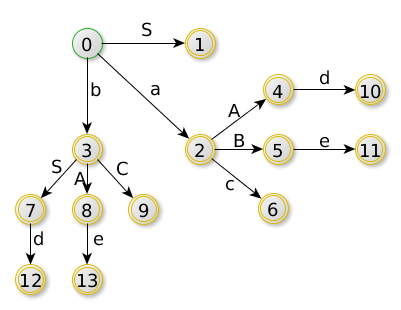
\includegraphics[scale=0.6]{Chapters/Img/c05_04.png}\\
\end{center}

0 =
\begin{tabular}{l}
	$S' \rightarrow .S,\  \{ \$ \}$		\\
	$S  \rightarrow .aAd,\  \{ \$ \}$	\\
	$S  \rightarrow .bBd,\  \{ \$ \}$	\\
	$S  \rightarrow .aBe,\  \{ \$ \}$	\\
	$S  \rightarrow .bAe,\  \{ \$ \}$	\\
\end{tabular}\\[5pt]

1 =
\begin{tabular}{l}
	$S' \rightarrow S.,\  \{ \$ \}$		\\
\end{tabular}\\[5pt]

2 =
\begin{tabular}{l}
	$S \rightarrow a.Ad  ,\  \{ \$ \}$	\\
	$S  \rightarrow a.Be ,\  \{ \$ \}$	\\
	$A  \rightarrow .c ,\  \{ d \}$	\\
	$B  \rightarrow .c ,\  \{ e \}$	\\
\end{tabular}\\[5pt]

3 =
\begin{tabular}{l}
	$S \rightarrow b.Bd  ,\  \{ \$ \}$	\\
	$S  \rightarrow b.Ae ,\  \{ \$ \}$	\\
	$B  \rightarrow .c ,\  \{ d \}$	\\
	$A  \rightarrow .c ,\  \{ e \}$	\\
\end{tabular}\\[5pt]

4 =
\begin{tabular}{l}
	$S \rightarrow aA.d ,\  \{ \$ \}$	\\
\end{tabular}\\[5pt]

5 =
\begin{tabular}{l}
	$S \rightarrow aB.e ,\  \{ \$ \}$	\\
\end{tabular}\\[5pt]

6 =
\begin{tabular}{l}
	$A \rightarrow c.,\  \{ d \}$	\\
	$B \rightarrow c.,\  \{ e \}$	\\
\end{tabular}\\[5pt]

7 =
\begin{tabular}{l}
	$S \rightarrow bB.d,\  \{ \$ \}$	\\
\end{tabular}\\[5pt]

8 =
\begin{tabular}{l}
	$S \rightarrow bA.e,\  \{ \$ \}$	\\
\end{tabular}\\[5pt]

9 =
\begin{tabular}{l}
	$B \rightarrow c.,\  \{ d \}$	\\
	$A \rightarrow c.,\  \{ e \}$	\\
\end{tabular}\\[5pt]

10 =
\begin{tabular}{l}
	$S \rightarrow aAd.,\  \{ \$ \}$	\\
\end{tabular}\\[5pt]

11 =
\begin{tabular}{l}
	$S \rightarrow aBe.,\  \{ \$ \}$	\\
\end{tabular}\\[5pt]

12 =
\begin{tabular}{l}
	$S \rightarrow bBd.,\  \{ \$ \}$	\\
\end{tabular}\\[5pt]

13 =
\begin{tabular}{l}
	$S \rightarrow bAe.,\  \{ \$ \}$	\\
\end{tabular}\\[5pt]

Gli stati 6 e 9 hanno la stessa proiezione quindi li mergio in \\

14 = 
\begin{tabular}{l}
	$A \rightarrow c.,\  \{ d \}$	\\
	$B \rightarrow c.,\  \{ e \}$	\\
	$A \rightarrow c.,\  \{ e \}$	\\
	$B \rightarrow c.,\  \{ d \}$	\\
\end{tabular}\\[5pt]

Sostituisco 14 a 6 e 9, faccio una transizione da 3 a 14

\begin{tabular}{|c|c|c|c|c|c|c|c|c|c|}
	\hline
		&	\textbf{a} 	& \textbf{b}	& \textbf{c}	& \textbf{d}	& \textbf{e} 	& $\bm{\$}$ & \textbf{S} & \textbf{A} & \textbf{B}	\\  
	\hline
	\textbf{0}	&	S2 	& S3 	& 		& 		&  	&  	& g1 &  & 	\\
	\hline
	\textbf{1}	&	 	&  	& 		& 		&  	&  ACC	&  &  & 	\\
	\hline
	\textbf{2}	&	 	&  	& 	S14	& 		&  	&  	&  &  g4  & g5	\\
	\hline
	\textbf{3}	&	 	&  	& 	S14	& 		&  	&  	&  &  g8  & g7	\\
	\hline
	\textbf{4}	&	 	&  	& 		& 	S10	&  	&  	&  &    & \\
	\hline
	\textbf{5}	&	 	&  	& 		& 		& S11  	&  	&  &    & 	\\
	\hline
	\textbf{7}	&	 	&  	& 		& 	S12	&   	&  	&  &   & 	\\
	\hline
	\textbf{8}	&	 	&  	& 		& 		& S13  	&  	&  &    & 	\\
	\hline
	\textbf{10}	&	 	&  	& 		& 		&   	& $S \rightarrow aAd$ 	&  &    & 	\\
	\hline
	\textbf{11}	&	 	&  	& 		& 		&   	& $S \rightarrow aBe$ 	&  &    & 	\\
	\hline
	\textbf{12}	&	 	&  	& 		& 		&   	& $S \rightarrow bBd$ 	&  &    & 	\\
	\hline
	\textbf{13}	&	 	&  	& 		& 		&   	& $S \rightarrow bAe$ 	&  &    & 	\\	
	\hline
	\textbf{14}	&	 	&  	& 		& 		& $A \rightarrow c \ B \rightarrow c$  	& $B \rightarrow c \ A \rightarrow c$ 	&  &    & 	\\	
	\hline
\end{tabular}

In 14 ho ancora dei conflitti reduce/reduce quindi la grammatica non \'e LALR.

\subsection{Esempio}
$S \rightarrow Ma | bMc | dc | bda$\\
$M \rightarrow d$\\

Non dovrebbe essere LALR perch\'e avrei $M \rightarrow d$ con lookahead set $\{ a \}\ e \{ d \}$...

\section{Algoritmo LALR (efficiente)}
\subsection{Esempio}

$S \rightarrow L = R | R$ \\
$L \rightarrow *R | id $ \\
$R \rightarrow L$ \\

\begin{center}
    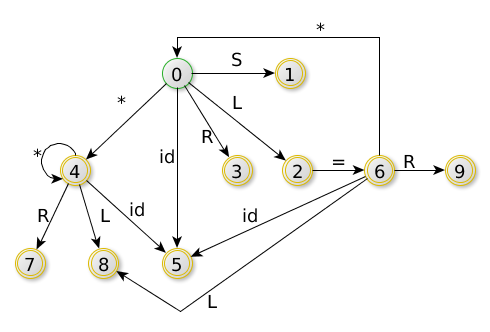
\includegraphics[scale=0.6]{Chapters/Img/c05_05.png}\\
\end{center}

0 = 
\begin{tabular}{l}
	$S' \rightarrow .S, \{ x_0 \}$\\
	$S \rightarrow .L, \{ x_0 \}$\\
	$S \rightarrow .R, \{ x_0 \}$\\
	$L \rightarrow .*R, \{ x_0 \}$\\
	$L \rightarrow .id, \{ x_0 \}$\\
	$R \rightarrow .L, \{ x_0 \}$\\
\end{tabular}\\[5pt]

1 = 
\begin{tabular}{l}
	$S' \rightarrow S., \{ x_1 \}$\\
\end{tabular}\\[5pt]

2 = 
\begin{tabular}{l}
	$S \rightarrow L. = R, \{ x_2 \}$\\
	$R \rightarrow L., \{ x_3 \}$\\
\end{tabular}\\[5pt]

3 = 
\begin{tabular}{l}
	$S \rightarrow R., \{ x_4 \}$\\
\end{tabular}\\[5pt]

4 = 
\begin{tabular}{l}
	$L \rightarrow *.R, \{ x_5 \}$\\
\end{tabular}\\[5pt]

5 = 
\begin{tabular}{l}
	$L \rightarrow id., \{ x_6 \}$\\
\end{tabular}\\[5pt]

6 = 
\begin{tabular}{l}
	$S \rightarrow L = .R, \{ x_7 \}$\\
	$R \rightarrow .L, \{ x_7 \}$\\
	$L \rightarrow .*R, \{ x_7 \}$\\
	$L \rightarrow .id, \{ x_7 \}$\\
\end{tabular}\\[5pt]

7 = 
\begin{tabular}{l}
	$L \rightarrow *R., \{ x_8 \}$\\
\end{tabular}\\[5pt]

8 = 
\begin{tabular}{l}
	$R \rightarrow L., \{ x_9 \}$\\
\end{tabular}\\[5pt]

9 = 
\begin{tabular}{l}
	$S \rightarrow L = R., \{ x_10 \}$\\
\end{tabular}\\[5pt]

$x_0 = \{ \$ \}$ \\
$x_1 = \{ x_0 \}$ \\
$x_2 = \{ x_0 \}$ \\
$x_3 = \{ x_0 \}$ \\
$x_4 = \{ x_0 \}$ \\
$x_5 = \{ \{ =, x_0 \} \cup \{ x_5 \} \cup \{ x_7 \} \}$  \\
$x_6 = \{ x_5 \}$ \\
$x_7 = \{ x_2 \}$ \\
$x_8 = \{ x_5 \}$ \\
$x_9 = \{ \{x_5\} \cup \{ x_7\} \}$ \\
$x_10 = \{ x_7 \}$ \\

Ora devo risolvere il sistema 
\begin{tabular}{ll}
		& 	\textbf{class} 	\\
	$x_0 = \{ \$ \}$	&	$x_0$ \\
	$x_1 $				&	$x_0$ \\
	$x_2 $				&	$x_0$ \\
	$x_3 $				&	$x_0$ \\
	$x_4 $				&	$x_0$ \\
	$x_5 = \{ =, x_0, x_5, x_7 \}$		&	$x_5$ \\
	$x_6 = \{ =, x_0, x_5, x_7 \}$		&	$x_6$ \\
	$x_7 $				&	$x_0$ \\
	$x_8 $				&	$x_5$ \\
	$x_9 = \{ x_5, x_7 \}$	&	$x_9$ \\
	$x_10$				&	$x_10$ \\
\end{tabular}

Mi rimangono quindi solo 4 variabili $x_0, x_5, x_6, x_9$
\begin{tabular}{ll} 
	$x_0 = \{ \$ \}$ 					& 	\\
	$x_5 = \{ =, x_0, x_5, x_7\$ \}$	& 	$= \{ =, x_0 \}$\\
	$x_6 = \{ =, x_0, x_5, x_7\$ \}$	& 	$= \{ =, x_0, x_5 \}$\\
	$x_9 = \{ x_5, x_7\$ \}$	& 	$= \{ x_5, x_0 \}$\\
\end{tabular}

Creo un grafo mettendo sui nodi le variabili, con solamente i terminali di quella variablie (non quelli presi dalle altre. Solo quelli che non sono $x_k$ insomma).

\begin{center}
    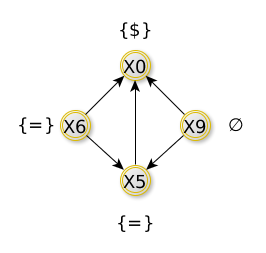
\includegraphics[scale=0.6]{Chapters/Img/c05_06.png}\\
\end{center}

Ottengo:
$x_0 = \{ \$ \}$ \\
$x_5 = \{ =, \$ \}$ \\
$x_6 = \{ =, \$ \}$ \\
$x_9 = \{ =, \$ \}$ \\

Questi sono il lookahead set che stavo cercando.

\begin{center}
    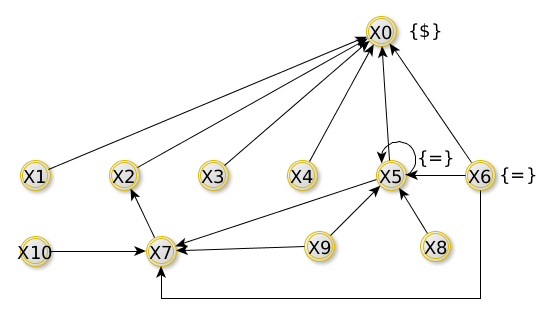
\includegraphics[scale=0.6]{Chapters/Img/c05_07.png}\\
\end{center}

\section{Costruzione automa simbolico}
\begin{lstlisting}
	x_0 = new Var();
	Vars = {x_0};
	P_0 =  closure1({[S' -> .S, {x_0}]});
	States = {P_0};
	P_0 unmarked;
	while(exists unmarked state P in States){
		mark P;
		foreach(Y in V){
			tmp = emptySet;
			foreach([A -> alpha . Y beta, delta] in P){
				tmp.Add(([A -> alpha . Y beta, delta]);
			}
			if(tmp is not empty){
				if(lo stato target non e'' ancora stato collezionato){
					States.Add(versione simbolica del target);
					Queue.Add(equazione per kernel item in tmp);
				} else {
					raffinare le equazioni delle variabili associate ai kernel item del target;
				}
			}
		}
	}
\end{lstlisting}

\section{Grammatiche Attribuite}

\begin{center}
	\begin{tabular}{ll}
		\textbf{SDD} & Syntax Directed Definition\\
		\textbf{SDT} & Syntax Directed Translation \\
	\end{tabular}
\end{center}

Una grammatica attribuita \'e una grammatica a cui sono aggiunti attributi e regole.\\[5pt]
$E \rightarrow E + T | T$\\
$T \rightarrow T * F | F$\\
$F \rightarrow (E) | id$\\
$w = 3+4*5$\

\begin{center}
    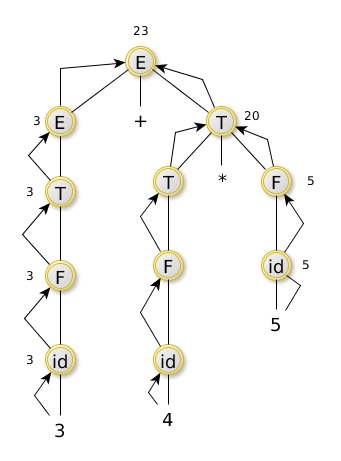
\includegraphics[scale=0.6]{Chapters/Img/c05_08.png}\\
\end{center}

Il valore di propaga dal basso verso l'alto nell'albero e computate le operazioni man mano che si presentano.\\[5pt]

\begin{tabular}{ll}
	$E_1 \rightarrow E_2 + T $ 		& 	$\{ E_1.val = E_2.val + T.val \}$	\\
	$E \rightarrow T $ 				& 	$\{ E.val = T.val \}$	\\
	$T_1 \rightarrow T_2 * F $ 		& 	$\{ T_1.val = T_2.val * F.val \}$	\\
	$T \rightarrow F $		 		& 	$\{ T.val = F.val \}$	\\
	$F \rightarrow E $		 		& 	$\{ F.valE = E.val \}$	\\
	$F \rightarrow id $ 			& 	$\{ F.val = lexval(id) \}$	\\
\end{tabular}
$\leftarrow$ Azione semantica \\[5pt]

L'abstract syntax tree di questa grammatica \'e:

\begin{center}
    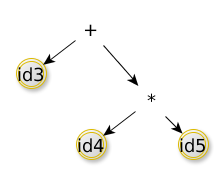
\includegraphics[scale=0.6]{Chapters/Img/c05_09.png}\\
\end{center}

\section{Attributi Sintetizzati ed Ereditati}
$A \rightarrow \alpha$ A.a definito come una funzione degli attributi dei terminali e non terminali in $\alpha$. Gli attributi dei terminali sono informazioni ottenute 
durante l'analisi lessicale.

\subsection{Esempio}
\begin{tabular}{ll}
	$D \rightarrow TL$ 			&	$ \{ L.i = T.t \} $\\
	$T \rightarrow int$ 		&	$ \{ T.t = integer \} $\\
	$T \rightarrow float $ 		&	$ \{ T.t = float \} $\\
	$L_1 \rightarrow L_2,\ id$ 	&	$ \{ L_2.i = L_1.i; addType(lexval(id), L_1.i) \} $\\
	$L \rightarrow id$ 			&	$ \{ addType(lexval(id), L_i) \} $\\
\end{tabular}

w = int pluto, pippo, paperino 

\begin{center}
    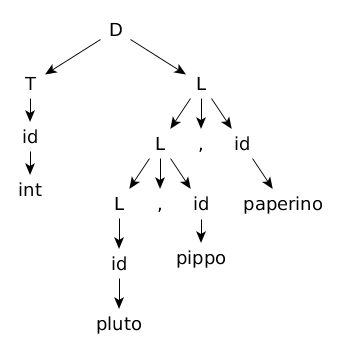
\includegraphics[scale=0.6]{Chapters/Img/c05_10.png}\\
\end{center}

Facendo bottom-up la prima cosa che faremo sar\'a $T \rightarrow int$. A questo punto T conosce \lq\lq int\rq\rq\ e lo dice alla L pi\'u in alto (quella subito sotto a D).
Quella L lo dice alla L sotto di lui, e questo succede anche per il livello dopo. Adesso L va ad \lq\lq id\rq\rq\ che diventa \lq\lq pluto\rq\rq\, che L viene a conoscere
(poich\'e viene passato in alto). Visto che alcuni attributi dipendono dai padri e dagli attributi dei fratelli, questi sono attributi ereditati.

Gli attributi ereditati sono funzione degli attributi di siblings e del padre.

\subsection{Esempio}
$S \rightarrow N$\\
$N \rightarrow o\ Digist$\\
$N \rightarrow Digits$\\
$Digits \rightarrow Digits\ d$\\
$Digits \rightarrow d$\\

Questo albero \'e simile a quello di prima: c\'e solo \lq\lq o\rq\rq\ a sinistra e potenzialmente infinite \lq\lq Digits\rq\rq\ a destra, una sotto l'altra.
Come fare per essere in grado di distinguere se c\'e la \lq\lq o\rq\rq\ oppure no?

Posso ribaltare l'albero, riscrivendo la grammatica come:\\
\begin{tabular}{ll}
	$S \rightarrow Digits$ 	&	$\{ Digits.qualcosa \}$\\
	$Digits_1 \rightarrow Digits_2 \ d $ 	&	$\{ Digits_1.val = Digits_2.val * Digits_2.base + 'd' \}$\\
	$Digits \rightarrow d $ 	&	$\{ Digits.base = 8;\ Digits.val = 'd' \}$\\
	$Digits \rightarrow od $ 	&	$\{ Digits.base = 10;\ Digits.val = 'd' \}$\\
\end{tabular}

%\chapter{14/11/17}
LALR(1)
LR(1)

\section{LRm(1)}
\subsection{Esempio}
\begin{tabular}{l}
	$S \rightarrow L=R|R$\\
	$L \rightarrow *R|id$\\
	$R \rightarrow L $\\
\end{tabular}
Lo stato iniziale \'e associato ad una variabile; ottenuto come chiusura (considero gli item LR(1)) 
$S' \rightarrow .S_1\{x_0\}$. \\

\subsubsection{Procedo con la chiusura LR(1)} 
\begin{tabular}{l}
	Equazioni\\
	$x_0 \doteq \{ \$ \}$\\
	$x_1 \doteq \{ x_0 \}$\\
	$x_1 \doteq x_0$\\
	$x_2 \doteq x_0$\\
	$x_3 \doteq x_0$\\
	$x_4 \doteq x_0$\\
	$x_5 \doteq \{ =, x_0 \} \cup \{ x_5 \} \cup \{ x_7 \}$\\
	$x_6 \doteq \{ =, x_0 \} \cup \{ x_5 \} \cup \{ x_7 \}$\\
	$x_7 \doteq \{ x_2 \}$\\
	$x_8 \doteq \{ x_5 \}$\\
	$x_9 \doteq \{ x_5 \} \cup \{ x_7 \}$\\
	$x_10 \doteq \{ x_7 \}$\\
\end{tabular}

\begin{tabular}{l}
	0) Stato 0-esimo
	$S' \rightarrow .S, \{ x_0 \}$\\
	...........................\\
	$S \rightarrow .L=R,\ \{x_0\}$\\
	$S \rightarrow .R,\ \{x_0\}$\\
	$L \rightarrow .*R,\ \{=, x_0\}$\\
	$L \rightarrow .id,\ \{=, x_0\}$\\
	$R \rightarrow .L,\ \{x_0\}$\\
\end{tabular}

\begin{tabular}{l}
	1) Transizione su S ($\rightarrow S$)\\
	$S' \rightarrow S.,\{ x_1 \}$\\
\end{tabular}

\begin{tabular}{l}
	2) Transizione su L\\
	$S \rightarrow L.=R, \{ x_2 \}$\\
	$R \rightarrow L., \{ x_3 \}$\\
\end{tabular}

\begin{tabular}{l}
	3) Transizione su R\\
	$S \rightarrow R., \{ x_4 \}$\\
\end{tabular}

\begin{tabular}{l}
	4) Transizione su *\\
	$L \rightarrow *.R, \{ x_5 \}$\\
	..............................
	$R \rightarrow .L, \{ x_5 \}$\\
	$R \rightarrow .*R, \{ x_5 \}$\\
	$R \rightarrow .id, \{ x_5 \}$\\
\end{tabular}

\begin{tabular}{l}
	5) Transizione su id\\
	$L \rightarrow id., \{ x_6 \}$\\
\end{tabular}

\begin{tabular}{l}
	6) Transizione da 2 su =\\
	$S \rightarrow L=.R, \{ x_7 \}$\\
	...............................\\
	$R \rightarrow .L, \{ x_7 \}$\\
	$L \rightarrow .*R, \{ x_7 \}$\\
	$L \rightarrow .id, \{ x_7 \}$\\
\end{tabular}

\begin{tabular}{l}
	7) Transizione da 4 su R\\
	$L \rightarrow *R., \{ x_8 \}$\\
\end{tabular}

\begin{tabular}{l}
	8) Transizione da 4 su L\\
	$R \rightarrow L., \{ x_9 \}$\\
	Ho un loop sullo stato 4 su * (transizione da 4 in 4)\\
\end{tabular}

\begin{tabular}{l}
	9) Transizione da 6 su R\\
	$S \rightarrow L=R., \{ x_10 \}$\\
	Inserire una L transizione da 6 a 8\\
	Inserire una * transizione da 6 a 4\\
	Inserire una id transizione da 6 a 5\\
\end{tabular}

\begin{tabular}{l}
	Equazioni\\
	$x_0 \doteq \{ \$ \}$\\
	$x_1 \doteq \{ x_0 \}$\\
	$x_1 \doteq x_0$\\
	$x_2 \doteq x_0$\\
	$x_3 \doteq x_0$\\
	$x_4 \doteq x_0$\\
	$x_5 \doteq \{ =, x_0 \} \cup \{ x_5 \} \cup \{ x_7 \}$\\
	$x_6 \doteq \{ =, x_0 \} \cup \{ x_5 \} \cup \{ x_7 \}$\\
	$x_7 \doteq \{ x_2 \}$\\
	$x_8 \doteq \{ x_5 \}$\\
	$x_9 \doteq \{ x_5 \} \cup \{ x_7 \}$\\
	$x_10 \doteq \{ x_7 \}$\\
\end{tabular}

\begin{tcolorbox}\begin{center}
	Controllo le equazioni dalla prima all'ultima e guardo se l'inisieme di destra ho una sola variabile o due di cui una il nodo di destra (self loop).
\end{center}\end{tcolorbox}

	$x_j = \{ x_i \} \cup \{ x_j \} = \{ x_i \}$\\
\begin{tabular}{ll}
	equazione & classe di equivalenza\\
	$x_0 = \{ \$ \}$ & $x_0$\\
	$x_1$ & $x_0$\\
	$x_2$ & $x_0$\\
	$x_3$ & $x_0$\\
	$x_4$ & $x_0$\\

	$x_5 = \{ =, x_0, x_5, x_7 \}$ & $ x_5 $\\
	$x_6 = \{ =, x_0, x_5, x_7 \}$ & $x_0$\\
	$x_7 = \{ \$ \}$ & $ x_6 $\\
	$x_8$ & $x_5$\\
	$x_9$ & $x_0$\\
	$x_10$ & $x_5$\\
\end{tabular}

\begin{tabular}{l}
	$x_0 = \$ $\\
	$x_5 = \{ =, x_0, x_5, x_7 \}$\\
	$x_6 = \{ =, x_0, x_5, x_7 \}$\\
	$x_9 = \{ x_5, x_7 \}$\\
\end{tabular}

\begin{tabular}{l}
	Tolgo i self loop e ridondanze
	$x_0 = \$ $\\
	$x_5 = \{ =, x_0 \}$\\
	$x_6 = \{ =, x_0, x_5 \}$ ($x_7 = x_0$, lo tolgo)\\
	$x_9 = \{ x_5, x_0 \}$\\
\end{tabular}

\begin{center}
	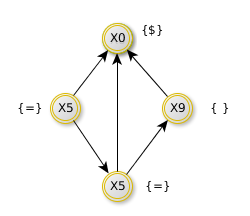
\includegraphics[scale=0.6]{Chapters/Img/l01_01.png}\\
\end{center} 

\begin{tabular}{l}
	$x_0 = \{ \$ \}$\\
	$x_5 = \{ =, \$ \}$\\
	$x_6 = \{ =, \$ \}$\\
	$x_9 = \{ =, \$ \}$\\
\end{tabular}

\section{Algoritmo}
Algoritmo utilizzato da yacc (su dragonbook)
Uso LR0, per ogni item dentro uno stato faccio una chiusura virtuale LR1
Faccio un nuovo grafo e ...

Identifica look ahead generati e propagati, poi fa un grafo e associa ad ogni nodo il look ahead generato

\begin{center}
	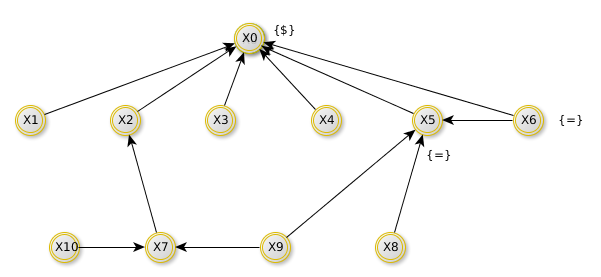
\includegraphics[scale=0.6]{Chapters/Img/l01_02.png}\\
\end{center} 

\begin{tcolorbox}\begin{center}
	Kernel(P) L'insiseme dei kernel item dentro P, proj(P) L'inisieme degli item LR(0) contenuti in P
\end{center}\end{tcolorbox}

\section{Costruzione automa simbolico}
\begin{lstlisting}
	x_0 = new Var()
	vars = {x_0}
	P_0 = closure_1( { [s' -> .s, {x_0} ] } ) //stato iniziale automa
	inizializzare Queue con x_0 = {$}
	States = {P_0}
	porre P_0 come unmarked
	while(c'e' uno stato non marcato P in States){
		marcare P
		foreach(y in V){
			Tmp = emptySet
			foreach([A -> alpha.y beta, delta] <- P){
				aggiungere [A -> alpha.y beta, delta] a Tmp
				if(Tmp != emptySet){
					if( lo stato targhet non e' ancora stato collezionato){
						aggiungere a States una versione simbolica del targhet e aggiungere a Queue una equazione per kernel item in Tmp
					} else {
						raffinare le equazioni delle variabili associate ai kernel item del target
					}
				}
			}
		}
	}
\end{lstlisting}


%\section{Grammatiche Attribute}
SDD (Syntax Directed Definition)
SDT (Syntax Directed Translation)

Aggiungo alla grammatica degli attributi e delle regole per quest'utlimi.
(Desc Calculator) posso computare valori associati ad espressioni aritmetiche.

%%%%%%%%%%%%%%%%%%%%%%%%%%%%%%%%%%%%%%%%%%%%%%%%%%%%%%%%%%%%%%%%%%%%%%%%%%%%
\subsection{Esempio}
\begin{tabular}{l}
	$E \rightarrow E + T | T$\\
	$T \rightarrow T * F | F$\\
	$F \rightarrow (E) | id$\\
\end{tabular}

Associo attributi ai terminali e non terminali, che recupero dall'analisi lessicale.

\begin{center}
	$3 + 4 * 5$ \\
	\Tree[. E [.E [.T [.F [.id (3) ] ] ] ] + [.T [.T [.F [.id (4) ] ] ] * [.F [.id (5) ] ] ] ]\\
\end{center}


Faccio visita postorder dell'albero (Bottom Up), associo i valori degli attributi a id, poi a F, poi risalgo a T. Quando sonon in T * F, T=4, F=5;
Quindi risolvo 4*5 che assegno come attributo al nodo padre T.

\begin{tcolorbox}\begin{center}
	\textbf{E.val} per indicare l'attributo della E.
\end{center}\end{tcolorbox}

\begin{tabular}{ll}
	$ \$\$ $ 	& Il driver\\
	$ \$ 1 $	& Primo elemento della produzione\\
\end{tabular}	 

$E_1 \rightarrow E_2 + T$ $\{ E_1.val = E_2.val + T.val \} $ \textbf{azione semantica} \\
$E \rightarrow T$ $\{ E.val = T.val \} $ \\
$T_1 \rightarrow T_2 * F $ $\{ T_1.val = T_2.val + F.val \} $ \\
$T \rightarrow F $ $ T.val = F.val $ \\
$F \rightarrow (E) $ $\{ F.val = E.val \} $ \\
$F \rightarrow id $ $\{ F.val = lexval(id) \} $ \\

Abstract Syntax Tree (albero derivazione \lq\lq ristretto\rq\rq )
\Tree[.+ $id_3$ [.* $id_4$ $id_5$ ] ]

\subsection{Attributi sintetizzati}
$A \rightarrow \alpha $ A.a definito come una funzione degli attributi dei terminali e non terminali in $\alpha $.
Gli attributi dei terminali derivano dall'analisi lessicale.

\subsection{Esempio, dichiarazione variabili}
\begin{lstlisting}
	int pippo, pluto, paperino;
\end{lstlisting}

$D \rightarrow TL$ $\{ L.i = T.t \} $\\
$T \rightarrow int$ $\{ T.t = integer\} $\\
$T \rightarrow float$ $\{ T.t = float \} $\\
$L_1 \rightarrow L_2,\ id$ $\{ L_2.i = L_1.i,\ addType(lex(id), L_1.i) \} $\\
$L \rightarrow id$ $\{ addType(lex(id)),\ L_i) \} $\\

\Tree[.D [.T int ] [.L [.L [.L [.id (pluto) ] ] , [.id (pippo) ] ] , [.id (paperino) ] ] ]

\begin{center}
	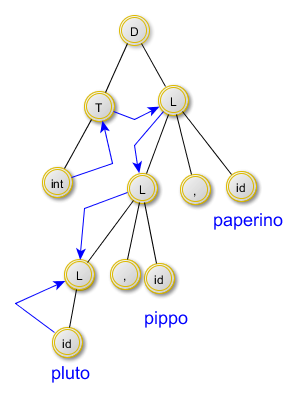
\includegraphics[scale=0.5]{Chapters/Img/l02_01.png}\\
\end{center} 

Gli attributi ereditati sono funzione degli attributi di siblings e del padre (driver della produzione).

\subsection{Example}
$S \rightarrow Number$\\
$Number \rightarrow o Digits$ serie di cifre in ottali (o)\\
$Number \rightarrow Digits d$\\
$Digits \rightarrow d$\\

\Tree[.N o [.Digits [.(...) d ] d ] ]

Gira l'albero!
$ S \rightarrow Digits $\\
$ Digits_1 \rightarrow Digits_2 d $ $\{ Digits_1.val = Digits_2 * Dg.tg_2.base + "d" \}$\\
$ Digits \rightarrow d $ $\{ Digit.base = 10; Digit.val = "d" \}$\\
$ Digits \rightarrow od $ $\{ Digit.base = 8; Digit.val = "d" \}$\\

Supponiamo per assurdo che sia LALR.
\end{document}